% Chapter 0: Introduction: components and exponential smoothing
% Time Series Analysis -- Bachelor's programmes Economic Informatics and Economic Cybernetics, Bucharest University of Economic Studies
% GENERATED by latex/build_chapter0.py -- edit the generator, not this file.

\newcommand{\coursename}{Time Series Analysis}
% Preambul comun TSA -- Serii de timp / Time Series Analysis (Beamer, 16:9)
% Același design ca MFM și SFM (preluat din SFM, 5 octombrie 2026). Înainte de % Preambul comun TSA -- Serii de timp / Time Series Analysis (Beamer, 16:9)
% Același design ca MFM și SFM (preluat din SFM, 5 octombrie 2026). Înainte de % Preambul comun TSA -- Serii de timp / Time Series Analysis (Beamer, 16:9)
% Același design ca MFM și SFM (preluat din SFM, 5 octombrie 2026). Înainte de \input{../../latex/preamble} se definește
%   \newcommand{\coursename}{Time Series Analysis}      (EN)
%   \newcommand{\coursename}{Serii de timp}       (RO)  și  \def\tsalang{ro}
% Fișierele .tex se află în EN/Courses, EN/Seminars, RO/Cursuri, RO/Seminarii (două niveluri sub rădăcină).
% Deck-urile sînt generate de latex/build_chapterN.py / build_seminarN.py (vezi latex/tsa_build.py).

\documentclass[9pt, aspectratio=169, t]{beamer}
\providecommand{\coursename}{Time Series Analysis}

% Ensure content fits on slides
\setbeamersize{text margin left=8mm, text margin right=8mm}
% Smaller institute font (title page)
\setbeamerfont{institute}{size=\footnotesize}

%=============================================================================
% THEME AND STYLE CONFIGURATION
%=============================================================================
\usetheme{default}
% Using default theme for clean header/footer control

% Color Palette (matching Redispatch PDF)
\definecolor{MainBlue}{RGB}{26, 58, 110}
\definecolor{AccentBlue}{RGB}{26, 58, 110}
\definecolor{IDAred}{RGB}{205, 0, 0}
\definecolor{DarkGray}{RGB}{51, 51, 51}
\definecolor{MediumGray}{RGB}{128, 128, 128}
\definecolor{LightGray}{RGB}{248, 248, 248}
\definecolor{VeryLightGray}{RGB}{235, 235, 235}
\definecolor{KeynoteGray}{RGB}{218, 218, 218}
\definecolor{SectionGray}{RGB}{120, 120, 120}
\definecolor{FooterGray}{RGB}{100, 100, 100}
\definecolor{Crimson}{RGB}{220, 53, 69}
\definecolor{Forest}{RGB}{46, 125, 50}
\definecolor{Amber}{RGB}{181, 133, 63}
\definecolor{Orange}{RGB}{230, 126, 34}
\definecolor{Purple}{RGB}{142, 68, 173}

% Gradient background (exact Keynote 315° gradient: white to RGB 218,218,218)
\setbeamertemplate{background}{%
    \begin{tikzpicture}[remember picture, overlay]
        \shade[shading=axis, shading angle=315,
        top color=white, bottom color=KeynoteGray]
        (current page.south west) rectangle (current page.north east);
    \end{tikzpicture}%
}
% Fallback solid color for compatibility
\setbeamercolor{background canvas}{bg=}

\setbeamercolor{palette primary}{bg=MainBlue, fg=white}
\setbeamercolor{palette secondary}{bg=MainBlue!85, fg=white}
\setbeamercolor{palette tertiary}{bg=MainBlue!70, fg=white}
\setbeamercolor{structure}{fg=MainBlue}
\setbeamercolor{title}{fg=IDAred}
\setbeamercolor{frametitle}{fg=IDAred, bg=}
\setbeamercolor{block title}{bg=MainBlue, fg=white}
\setbeamercolor{block body}{bg=VeryLightGray, fg=DarkGray}
\setbeamercolor{block title alerted}{bg=Crimson, fg=white}
\setbeamercolor{block body alerted}{bg=Crimson!8, fg=DarkGray}
\setbeamercolor{block title example}{bg=Forest, fg=white}
\setbeamercolor{block body example}{bg=Forest!8, fg=DarkGray}
\setbeamercolor{item}{fg=MainBlue}

% Footer colors (override Madrid theme blue)
\setbeamercolor{author in head/foot}{fg=FooterGray, bg=}
\setbeamercolor{title in head/foot}{fg=FooterGray, bg=}
\setbeamercolor{date in head/foot}{fg=FooterGray, bg=}
\setbeamercolor{section in head/foot}{fg=FooterGray, bg=}
\setbeamercolor{subsection in head/foot}{fg=FooterGray, bg=}

% Bullet styles (apply everywhere including blocks)
\setbeamertemplate{itemize item}{\color{MainBlue}$\boxdot$}
\setbeamertemplate{itemize subitem}{\color{MainBlue}$\blacktriangleright$}
\setbeamertemplate{itemize subsubitem}{\color{MainBlue}\tiny$\bullet$}
\setbeamertemplate{itemize/enumerate body begin}{\normalsize}
\setbeamertemplate{itemize/enumerate subbody begin}{\normalsize}

% Item spacing - compact style
\setlength{\leftmargini}{10pt}       % Level 1: minimal indent
\setlength{\leftmarginii}{10pt}      % Level 2: minimal additional indent
% Compact list spacing (zero extra space before/after lists in blocks)
\makeatletter
\def\@listi{\leftmargin\leftmargini \topsep 0pt \parsep 0pt \itemsep 0pt}
\def\@listii{\leftmargin\leftmarginii \topsep 0pt \parsep 0pt \itemsep 0pt}
\makeatother

\setbeamertemplate{navigation symbols}{}

%=============================================================================
% CUSTOM HEADLINE
%=============================================================================
\setbeamertemplate{headline}{%
    \vskip10pt%
    \hbox to \paperwidth{%
        \hskip0.5cm%
        {\small\color{FooterGray}\renewcommand{\hyperlink}[2]{##2}\insertsectionhead}%
        \hfill%
        \textcolor{FooterGray}{\small\insertframenumber}%
        \hskip0.5cm%
    }%
    \vskip4pt%
    {\color{FooterGray}\hrule height 0.4pt}%
}

%=============================================================================
% CUSTOM FOOTER
%=============================================================================
\usepackage{fontawesome5}

\setbeamertemplate{footline}{%
    {\color{FooterGray}\hrule height 0.4pt}%
    \vskip4pt%
    \hbox to \paperwidth{%
        \hskip0.5cm%
        \textcolor{FooterGray}{\small\coursename}%
        \hfill%
        \raisebox{-0.1em}{%
            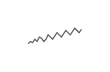
\begin{tikzpicture}[x=0.08em, y=0.08em, line width=0.4pt]
                \draw[FooterGray] (0,3) -- (1,4) -- (2,3.5) -- (3,5) -- (4,4) -- (5,6) -- (6,5.5) -- (7,4) -- (8,5) -- (9,7) -- (10,6) -- (11,5) -- (12,6.5) -- (13,8) -- (14,7) -- (15,6) -- (16,7.5) -- (17,9) -- (18,8) -- (19,7) -- (20,8.5) -- (21,10) -- (22,9) -- (23,8) -- (24,9.5);
            \end{tikzpicture}%
        }%
        \hskip0.5cm%
    }%
    \vskip6pt%
}

%=============================================================================
% PACKAGES
%=============================================================================
\usepackage[utf8]{inputenc}
\DeclareUnicodeCharacter{03B1}{\ensuremath{\alpha}}
\usepackage[T1]{fontenc}
\usepackage{amsmath, amssymb, amsthm}
\usepackage{mathtools}
\usepackage{bm}
\usepackage{tikz}
\usetikzlibrary{arrows.meta, positioning, shapes, calc, decorations.pathreplacing, shadings}
\usepackage{booktabs}
\usepackage{multirow}
\usepackage{array}
\usepackage{graphicx}
\usepackage{animate}
\usepackage{hyperref}
\usepackage{colortbl}
\usepackage{listings}
\lstset{language=Python, basicstyle=\ttfamily\scriptsize, keywordstyle=\color{MainBlue}\bfseries,
  commentstyle=\color{Forest}, stringstyle=\color{Crimson}, breaklines=true,
  frame=none, backgroundcolor=\color{VeryLightGray}, xleftmargin=2mm}
\hypersetup{colorlinks=true, linkcolor=MainBlue, urlcolor=MainBlue}
\graphicspath{{../../logos/}{../../charts/}{../../photos/}}
\usepackage{xcolor}
\hfuzz=2pt  % Suppress tiny overfull warnings (<2pt)
\vfuzz=2pt  % Suppress tiny vertical overfull warnings (<2pt)
% \mathrm in the sans-serif family of the slides (beamer resets \mathrm to the serif family at \begin{document};
% this hook runs after beamer's, so WN, Var, RMSE, ... in formulas match the surrounding text)
% Bold vectors and matrices in the same sans-serif family: \mathbf{A} in sans bold (beamer's own \mathbf came out in
% medium weight), and the bold upright Greek capitals of \boldsymbol / \bm (\bSigma, \bPhi, \boldsymbol{\Theta}) in
% cmss bold: bm.sty fixes its "boldoperators" font when it is loaded (serif cmbx), before beamer switches the
% operators to cmss, so it is reset here.
\AtBeginDocument{%
  \SetMathAlphabet{\mathrm}{normal}{\encodingdefault}{\sfdefault}{\mddefault}{n}%
  \SetMathAlphabet{\mathrm}{bold}{\encodingdefault}{\sfdefault}{bx}{n}%
  \SetMathAlphabet{\mathbf}{normal}{\encodingdefault}{\sfdefault}{bx}{n}%
  \SetMathAlphabet{\mathbf}{bold}{\encodingdefault}{\sfdefault}{bx}{n}%
  \SetSymbolFont{boldoperators}{normal}{OT1}{cmss}{bx}{n}%
  \SetSymbolFont{boldoperators}{bold}{OT1}{cmss}{bx}{n}}

%=============================================================================
% QUANTLET COMMANDS
%   \quantlet{<displayed name>}{<url>}       (generic, compatible with the older TSA decks)
%   \tsaquantlet{Ch_05}{TSA_ch5_garch}       -> https://github.com/danpele/Time-Series-Analysis/tree/main/Quantlets/Ch_05/TSA_ch5_garch
%   \qlurl{<folder>} is defined per chapter by the generator (Quantlets/Ch_NN/<folder>)
%=============================================================================
\newcommand{\tsarepo}{https://github.com/danpele/Time-Series-Analysis}
\newcommand{\tsaqlbase}{https://github.com/danpele/Time-Series-Analysis/tree/main/Quantlets}
\newcommand{\quantlet}[2]{%
    \hfill\href{#2}{%
        \raisebox{-0.15em}{
\includegraphics[height=0.7em]{ql_logo.png}}%
        \textcolor{MainBlue}{\tiny\ #1}%
    }%
}
\newcommand{\tsaquantlet}[2]{\quantlet{\detokenize{#2}}{\tsaqlbase/#1/#2}}

%=============================================================================
% NOTEBOOKS (Google Colab)
%   \colaburl{notebooks/EN/chapter5_seminar_notebook.ipynb} -> the Colab link of a file in the TSA repo
%   \nb: the chapter notebook (each seminar deck redefines it with \renewcommand)
%=============================================================================
\newcommand{\colaburl}[1]{https://colab.research.google.com/github/danpele/Time-Series-Analysis/blob/main/#1}
\newcommand{\nb}{https://colab.research.google.com/github/danpele/Time-Series-Analysis/tree/main/notebooks/EN}
\newcommand{\nbname}{notebooks/EN}

%=============================================================================
% SLIDE HELPERS (used by the generators; the same as in MFM)
%=============================================================================
% local font size for list bodies (the preamble forces \normalsize)
\newcommand{\itemsize}[1]{\setbeamertemplate{itemize/enumerate body begin}{#1}\setbeamertemplate{itemize/enumerate subbody begin}{#1}}
\newcommand{\intitle}[1]{{\hypersetup{urlcolor=white}#1}}   % white links inside coloured title bars
\newcommand{\imgcap}[1]{{\scriptsize #1}\\[0.5mm]}          % caption under a photo
\newcommand{\imgcredit}[2]{{\tiny\color{FooterGray}\href{#1}{#2}}}   % image credit: source URL, author/licence
\newcommand{\aiprompt}[1]{{\ttfamily\color{MainBlue}#1}}     % a prompt to an AI assistant

%=============================================================================
% SEMINARS: student version by default; the instructor wrapper *_solutions.tex sets \solutionstrue
%=============================================================================
\makeatletter\@ifundefined{ifsolutions}{\expandafter\newif\csname ifsolutions\endcsname}{}\makeatother
\newcommand{\solonly}[1]{\ifsolutions #1\fi}
\newcommand{\propsub}{\ifsolutions\else\framesubtitle{\ifdefined\tsalang Rezolvarea se discută la seminar\else Solution discussed in class\fi}\fi}

%=============================================================================
% APPENDIX AND CHAPTER LINKS (latex/appendix_links.py writes the calls; it also re-declares these
% macros before \begin{document}, so the decks compile with or without this preamble block)
%=============================================================================
\providecommand{\tsaapplink}[3]{\hypertarget{#2}{}\hyperlink{#1}{\beamergotobutton{#3}}}
\providecommand{\tsaappback}[2]{\begin{tikzpicture}[remember picture,overlay]\node[anchor=south east] at ([xshift=-3mm,yshift=7mm]current page.south east){\hyperlink{#1}{\beamerreturnbutton{#2}}};\end{tikzpicture}}
\providecommand{\tsachlink}[2]{\href{#1}{#2}}
\providecommand{\tsachlinkt}[2]{\href{#1}{\usebeamercolor[fg]{frametitle}#2}}

%=============================================================================
% QUANTINAR COMMAND: link către un curs Quantinar (subiecte avansate)
%=============================================================================
\newcommand{\quantinar}[2]{%
    \href{#2}{%
        \raisebox{-0.15em}{
\includegraphics[height=0.8em]{qr_logo.png}}%
        \textcolor{MainBlue}{\scriptsize\ #1}%
    }%
}

%=============================================================================
% CUSTOM TITLE PAGE
%=============================================================================
\defbeamertemplate*{title page}{hybrid}[1][]
{
    \vspace{0.2cm}
    % Logos row - top header (with clickable links)
    \begin{center}
        \href{https://www.ase.ro}{
\includegraphics[height=1.0cm]{ase_logo.png}}\hspace{0.3cm}%
        \href{https://theida.net}{
\includegraphics[height=1.0cm]{ida_logo.png}}\hspace{0.3cm}%
        \href{https://blockchain-research-center.com}{
\includegraphics[height=1.0cm]{brc_logo.png}}\hspace{0.3cm}%
        \href{https://www.ai4efin.ase.ro}{
\includegraphics[height=1.0cm]{ai4efin_logo.png}}\hspace{0.3cm}%
        \href{https://ipe.ro/new}{
\includegraphics[height=1.0cm]{acad_logo.png}}\hspace{0.3cm}%
        \href{https://www.digital-finance-msca.com}{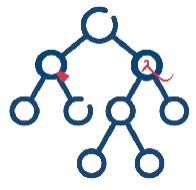
\includegraphics[height=1.0cm]{msca_logo.png}}%
    \end{center}

    \vspace{0.6cm}

    % Main title with Q logos on sides (with clickable links)
    \begin{center}
        \begin{minipage}{0.1\textwidth}
            \centering
            \href{https://quantlet.com}{
\includegraphics[height=1.1cm]{ql_logo.png}}
        \end{minipage}%
        \begin{minipage}{0.78\textwidth}
            \centering
            {\LARGE\bfseries\usebeamercolor[fg]{title}\inserttitle}

            \vspace{0.3cm}

            {\usebeamerfont{subtitle}\usebeamercolor[fg]{title}\insertsubtitle}
        \end{minipage}%
        \begin{minipage}{0.1\textwidth}
            \centering
            \href{https://quantinar.com}{
\includegraphics[height=1.1cm]{qr_logo.png}}
        \end{minipage}
    \end{center}

    \vspace{0.6cm}

    % Authors (left aligned)
    \hspace{0.5cm}{\usebeamerfont{author}\insertauthor}

    \vspace{0.3cm}

    % Institute/Affiliations (left aligned)
    \hspace{0.5cm}\begin{minipage}[t]{0.9\textwidth}
        \raggedright\small\insertinstitute
    \end{minipage}
}

%=============================================================================
% THEOREM ENVIRONMENTS
%=============================================================================
\theoremstyle{definition}
\setbeamertemplate{theorems}[numbered]
\ifdefined\tsalang
\newtheorem{defn}{Definiție}
\newtheorem{thm}{Teoremă}
\newtheorem{prop}{Propoziție}
\newtheorem{rmk}{Observație}
\else
\newtheorem{defn}{Definition}
\newtheorem{thm}{Theorem}
\newtheorem{prop}{Proposition}
\newtheorem{rmk}{Remark}
\fi

%=============================================================================
% CENTRED MINIPAGE (no extra vertical space)
%=============================================================================
\newenvironment{cminipage}[1]{%
    \par\noindent\hfill\begin{minipage}{#1}\ignorespaces
}{%
    \end{minipage}\hfill\null\par
}

%=============================================================================
% CUSTOM COMMANDS
%=============================================================================
\newcommand{\E}{\mathbb{E}}
\newcommand{\Var}{\text{Var}}
\newcommand{\Cov}{\text{Cov}}
\newcommand{\Corr}{\text{Corr}}
\newcommand{\R}{\mathbb{R}}
\newcommand{\N}{\mathbb{N}}
\newcommand{\Z}{\mathbb{Z}}
\newcommand{\B}{\mathbf{B}}
\newcommand{\imark}{\textcolor{MainBlue}{\textbullet}}
\newcommand{\RMSE}{\text{RMSE}}
\newcommand{\MAE}{\text{MAE}}
\newcommand{\MAPE}{\text{MAPE}}

% Boldface vector/matrix commands (VAR, VECM, state space; also used by the older TSA decks)
\newcommand{\bY}{\mathbf{Y}}
\newcommand{\bX}{\mathbf{X}}
\newcommand{\bA}{\mathbf{A}}
\newcommand{\bB}{\mathbf{B}}
\newcommand{\bepsilon}{\boldsymbol{\varepsilon}}
\newcommand{\bSigma}{\boldsymbol{\Sigma}}
\newcommand{\bPhi}{\boldsymbol{\Phi}}
\newcommand{\bGamma}{\boldsymbol{\Gamma}}
\newcommand{\bPi}{\boldsymbol{\Pi}}
\newcommand{\bc}{\mathbf{c}}
\newcommand{\balpha}{\boldsymbol{\alpha}}
\newcommand{\bbeta}{\boldsymbol{\beta}}
\newcommand{\bvarepsilon}{\boldsymbol{\varepsilon}}

% Legacy seminar marks (older TSA seminar decks)
\newcommand{\correct}{\textcolor{Forest}{\checkmark}}
\newcommand{\incorrect}{\textcolor{Crimson}{\texttimes}}
 se definește
%   \newcommand{\coursename}{Time Series Analysis}      (EN)
%   \newcommand{\coursename}{Serii de timp}       (RO)  și  \def\tsalang{ro}
% Fișierele .tex se află în EN/Courses, EN/Seminars, RO/Cursuri, RO/Seminarii (două niveluri sub rădăcină).
% Deck-urile sînt generate de latex/build_chapterN.py / build_seminarN.py (vezi latex/tsa_build.py).

\documentclass[9pt, aspectratio=169, t]{beamer}
\providecommand{\coursename}{Time Series Analysis}

% Ensure content fits on slides
\setbeamersize{text margin left=8mm, text margin right=8mm}
% Smaller institute font (title page)
\setbeamerfont{institute}{size=\footnotesize}

%=============================================================================
% THEME AND STYLE CONFIGURATION
%=============================================================================
\usetheme{default}
% Using default theme for clean header/footer control

% Color Palette (matching Redispatch PDF)
\definecolor{MainBlue}{RGB}{26, 58, 110}
\definecolor{AccentBlue}{RGB}{26, 58, 110}
\definecolor{IDAred}{RGB}{205, 0, 0}
\definecolor{DarkGray}{RGB}{51, 51, 51}
\definecolor{MediumGray}{RGB}{128, 128, 128}
\definecolor{LightGray}{RGB}{248, 248, 248}
\definecolor{VeryLightGray}{RGB}{235, 235, 235}
\definecolor{KeynoteGray}{RGB}{218, 218, 218}
\definecolor{SectionGray}{RGB}{120, 120, 120}
\definecolor{FooterGray}{RGB}{100, 100, 100}
\definecolor{Crimson}{RGB}{220, 53, 69}
\definecolor{Forest}{RGB}{46, 125, 50}
\definecolor{Amber}{RGB}{181, 133, 63}
\definecolor{Orange}{RGB}{230, 126, 34}
\definecolor{Purple}{RGB}{142, 68, 173}

% Gradient background (exact Keynote 315° gradient: white to RGB 218,218,218)
\setbeamertemplate{background}{%
    \begin{tikzpicture}[remember picture, overlay]
        \shade[shading=axis, shading angle=315,
        top color=white, bottom color=KeynoteGray]
        (current page.south west) rectangle (current page.north east);
    \end{tikzpicture}%
}
% Fallback solid color for compatibility
\setbeamercolor{background canvas}{bg=}

\setbeamercolor{palette primary}{bg=MainBlue, fg=white}
\setbeamercolor{palette secondary}{bg=MainBlue!85, fg=white}
\setbeamercolor{palette tertiary}{bg=MainBlue!70, fg=white}
\setbeamercolor{structure}{fg=MainBlue}
\setbeamercolor{title}{fg=IDAred}
\setbeamercolor{frametitle}{fg=IDAred, bg=}
\setbeamercolor{block title}{bg=MainBlue, fg=white}
\setbeamercolor{block body}{bg=VeryLightGray, fg=DarkGray}
\setbeamercolor{block title alerted}{bg=Crimson, fg=white}
\setbeamercolor{block body alerted}{bg=Crimson!8, fg=DarkGray}
\setbeamercolor{block title example}{bg=Forest, fg=white}
\setbeamercolor{block body example}{bg=Forest!8, fg=DarkGray}
\setbeamercolor{item}{fg=MainBlue}

% Footer colors (override Madrid theme blue)
\setbeamercolor{author in head/foot}{fg=FooterGray, bg=}
\setbeamercolor{title in head/foot}{fg=FooterGray, bg=}
\setbeamercolor{date in head/foot}{fg=FooterGray, bg=}
\setbeamercolor{section in head/foot}{fg=FooterGray, bg=}
\setbeamercolor{subsection in head/foot}{fg=FooterGray, bg=}

% Bullet styles (apply everywhere including blocks)
\setbeamertemplate{itemize item}{\color{MainBlue}$\boxdot$}
\setbeamertemplate{itemize subitem}{\color{MainBlue}$\blacktriangleright$}
\setbeamertemplate{itemize subsubitem}{\color{MainBlue}\tiny$\bullet$}
\setbeamertemplate{itemize/enumerate body begin}{\normalsize}
\setbeamertemplate{itemize/enumerate subbody begin}{\normalsize}

% Item spacing - compact style
\setlength{\leftmargini}{10pt}       % Level 1: minimal indent
\setlength{\leftmarginii}{10pt}      % Level 2: minimal additional indent
% Compact list spacing (zero extra space before/after lists in blocks)
\makeatletter
\def\@listi{\leftmargin\leftmargini \topsep 0pt \parsep 0pt \itemsep 0pt}
\def\@listii{\leftmargin\leftmarginii \topsep 0pt \parsep 0pt \itemsep 0pt}
\makeatother

\setbeamertemplate{navigation symbols}{}

%=============================================================================
% CUSTOM HEADLINE
%=============================================================================
\setbeamertemplate{headline}{%
    \vskip10pt%
    \hbox to \paperwidth{%
        \hskip0.5cm%
        {\small\color{FooterGray}\renewcommand{\hyperlink}[2]{##2}\insertsectionhead}%
        \hfill%
        \textcolor{FooterGray}{\small\insertframenumber}%
        \hskip0.5cm%
    }%
    \vskip4pt%
    {\color{FooterGray}\hrule height 0.4pt}%
}

%=============================================================================
% CUSTOM FOOTER
%=============================================================================
\usepackage{fontawesome5}

\setbeamertemplate{footline}{%
    {\color{FooterGray}\hrule height 0.4pt}%
    \vskip4pt%
    \hbox to \paperwidth{%
        \hskip0.5cm%
        \textcolor{FooterGray}{\small\coursename}%
        \hfill%
        \raisebox{-0.1em}{%
            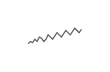
\begin{tikzpicture}[x=0.08em, y=0.08em, line width=0.4pt]
                \draw[FooterGray] (0,3) -- (1,4) -- (2,3.5) -- (3,5) -- (4,4) -- (5,6) -- (6,5.5) -- (7,4) -- (8,5) -- (9,7) -- (10,6) -- (11,5) -- (12,6.5) -- (13,8) -- (14,7) -- (15,6) -- (16,7.5) -- (17,9) -- (18,8) -- (19,7) -- (20,8.5) -- (21,10) -- (22,9) -- (23,8) -- (24,9.5);
            \end{tikzpicture}%
        }%
        \hskip0.5cm%
    }%
    \vskip6pt%
}

%=============================================================================
% PACKAGES
%=============================================================================
\usepackage[utf8]{inputenc}
\DeclareUnicodeCharacter{03B1}{\ensuremath{\alpha}}
\usepackage[T1]{fontenc}
\usepackage{amsmath, amssymb, amsthm}
\usepackage{mathtools}
\usepackage{bm}
\usepackage{tikz}
\usetikzlibrary{arrows.meta, positioning, shapes, calc, decorations.pathreplacing, shadings}
\usepackage{booktabs}
\usepackage{multirow}
\usepackage{array}
\usepackage{graphicx}
\usepackage{animate}
\usepackage{hyperref}
\usepackage{colortbl}
\usepackage{listings}
\lstset{language=Python, basicstyle=\ttfamily\scriptsize, keywordstyle=\color{MainBlue}\bfseries,
  commentstyle=\color{Forest}, stringstyle=\color{Crimson}, breaklines=true,
  frame=none, backgroundcolor=\color{VeryLightGray}, xleftmargin=2mm}
\hypersetup{colorlinks=true, linkcolor=MainBlue, urlcolor=MainBlue}
\graphicspath{{../../logos/}{../../charts/}{../../photos/}}
\usepackage{xcolor}
\hfuzz=2pt  % Suppress tiny overfull warnings (<2pt)
\vfuzz=2pt  % Suppress tiny vertical overfull warnings (<2pt)
% \mathrm in the sans-serif family of the slides (beamer resets \mathrm to the serif family at \begin{document};
% this hook runs after beamer's, so WN, Var, RMSE, ... in formulas match the surrounding text)
% Bold vectors and matrices in the same sans-serif family: \mathbf{A} in sans bold (beamer's own \mathbf came out in
% medium weight), and the bold upright Greek capitals of \boldsymbol / \bm (\bSigma, \bPhi, \boldsymbol{\Theta}) in
% cmss bold: bm.sty fixes its "boldoperators" font when it is loaded (serif cmbx), before beamer switches the
% operators to cmss, so it is reset here.
\AtBeginDocument{%
  \SetMathAlphabet{\mathrm}{normal}{\encodingdefault}{\sfdefault}{\mddefault}{n}%
  \SetMathAlphabet{\mathrm}{bold}{\encodingdefault}{\sfdefault}{bx}{n}%
  \SetMathAlphabet{\mathbf}{normal}{\encodingdefault}{\sfdefault}{bx}{n}%
  \SetMathAlphabet{\mathbf}{bold}{\encodingdefault}{\sfdefault}{bx}{n}%
  \SetSymbolFont{boldoperators}{normal}{OT1}{cmss}{bx}{n}%
  \SetSymbolFont{boldoperators}{bold}{OT1}{cmss}{bx}{n}}

%=============================================================================
% QUANTLET COMMANDS
%   \quantlet{<displayed name>}{<url>}       (generic, compatible with the older TSA decks)
%   \tsaquantlet{Ch_05}{TSA_ch5_garch}       -> https://github.com/danpele/Time-Series-Analysis/tree/main/Quantlets/Ch_05/TSA_ch5_garch
%   \qlurl{<folder>} is defined per chapter by the generator (Quantlets/Ch_NN/<folder>)
%=============================================================================
\newcommand{\tsarepo}{https://github.com/danpele/Time-Series-Analysis}
\newcommand{\tsaqlbase}{https://github.com/danpele/Time-Series-Analysis/tree/main/Quantlets}
\newcommand{\quantlet}[2]{%
    \hfill\href{#2}{%
        \raisebox{-0.15em}{
\includegraphics[height=0.7em]{ql_logo.png}}%
        \textcolor{MainBlue}{\tiny\ #1}%
    }%
}
\newcommand{\tsaquantlet}[2]{\quantlet{\detokenize{#2}}{\tsaqlbase/#1/#2}}

%=============================================================================
% NOTEBOOKS (Google Colab)
%   \colaburl{notebooks/EN/chapter5_seminar_notebook.ipynb} -> the Colab link of a file in the TSA repo
%   \nb: the chapter notebook (each seminar deck redefines it with \renewcommand)
%=============================================================================
\newcommand{\colaburl}[1]{https://colab.research.google.com/github/danpele/Time-Series-Analysis/blob/main/#1}
\newcommand{\nb}{https://colab.research.google.com/github/danpele/Time-Series-Analysis/tree/main/notebooks/EN}
\newcommand{\nbname}{notebooks/EN}

%=============================================================================
% SLIDE HELPERS (used by the generators; the same as in MFM)
%=============================================================================
% local font size for list bodies (the preamble forces \normalsize)
\newcommand{\itemsize}[1]{\setbeamertemplate{itemize/enumerate body begin}{#1}\setbeamertemplate{itemize/enumerate subbody begin}{#1}}
\newcommand{\intitle}[1]{{\hypersetup{urlcolor=white}#1}}   % white links inside coloured title bars
\newcommand{\imgcap}[1]{{\scriptsize #1}\\[0.5mm]}          % caption under a photo
\newcommand{\imgcredit}[2]{{\tiny\color{FooterGray}\href{#1}{#2}}}   % image credit: source URL, author/licence
\newcommand{\aiprompt}[1]{{\ttfamily\color{MainBlue}#1}}     % a prompt to an AI assistant

%=============================================================================
% SEMINARS: student version by default; the instructor wrapper *_solutions.tex sets \solutionstrue
%=============================================================================
\makeatletter\@ifundefined{ifsolutions}{\expandafter\newif\csname ifsolutions\endcsname}{}\makeatother
\newcommand{\solonly}[1]{\ifsolutions #1\fi}
\newcommand{\propsub}{\ifsolutions\else\framesubtitle{\ifdefined\tsalang Rezolvarea se discută la seminar\else Solution discussed in class\fi}\fi}

%=============================================================================
% APPENDIX AND CHAPTER LINKS (latex/appendix_links.py writes the calls; it also re-declares these
% macros before \begin{document}, so the decks compile with or without this preamble block)
%=============================================================================
\providecommand{\tsaapplink}[3]{\hypertarget{#2}{}\hyperlink{#1}{\beamergotobutton{#3}}}
\providecommand{\tsaappback}[2]{\begin{tikzpicture}[remember picture,overlay]\node[anchor=south east] at ([xshift=-3mm,yshift=7mm]current page.south east){\hyperlink{#1}{\beamerreturnbutton{#2}}};\end{tikzpicture}}
\providecommand{\tsachlink}[2]{\href{#1}{#2}}
\providecommand{\tsachlinkt}[2]{\href{#1}{\usebeamercolor[fg]{frametitle}#2}}

%=============================================================================
% QUANTINAR COMMAND: link către un curs Quantinar (subiecte avansate)
%=============================================================================
\newcommand{\quantinar}[2]{%
    \href{#2}{%
        \raisebox{-0.15em}{
\includegraphics[height=0.8em]{qr_logo.png}}%
        \textcolor{MainBlue}{\scriptsize\ #1}%
    }%
}

%=============================================================================
% CUSTOM TITLE PAGE
%=============================================================================
\defbeamertemplate*{title page}{hybrid}[1][]
{
    \vspace{0.2cm}
    % Logos row - top header (with clickable links)
    \begin{center}
        \href{https://www.ase.ro}{
\includegraphics[height=1.0cm]{ase_logo.png}}\hspace{0.3cm}%
        \href{https://theida.net}{
\includegraphics[height=1.0cm]{ida_logo.png}}\hspace{0.3cm}%
        \href{https://blockchain-research-center.com}{
\includegraphics[height=1.0cm]{brc_logo.png}}\hspace{0.3cm}%
        \href{https://www.ai4efin.ase.ro}{
\includegraphics[height=1.0cm]{ai4efin_logo.png}}\hspace{0.3cm}%
        \href{https://ipe.ro/new}{
\includegraphics[height=1.0cm]{acad_logo.png}}\hspace{0.3cm}%
        \href{https://www.digital-finance-msca.com}{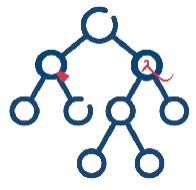
\includegraphics[height=1.0cm]{msca_logo.png}}%
    \end{center}

    \vspace{0.6cm}

    % Main title with Q logos on sides (with clickable links)
    \begin{center}
        \begin{minipage}{0.1\textwidth}
            \centering
            \href{https://quantlet.com}{
\includegraphics[height=1.1cm]{ql_logo.png}}
        \end{minipage}%
        \begin{minipage}{0.78\textwidth}
            \centering
            {\LARGE\bfseries\usebeamercolor[fg]{title}\inserttitle}

            \vspace{0.3cm}

            {\usebeamerfont{subtitle}\usebeamercolor[fg]{title}\insertsubtitle}
        \end{minipage}%
        \begin{minipage}{0.1\textwidth}
            \centering
            \href{https://quantinar.com}{
\includegraphics[height=1.1cm]{qr_logo.png}}
        \end{minipage}
    \end{center}

    \vspace{0.6cm}

    % Authors (left aligned)
    \hspace{0.5cm}{\usebeamerfont{author}\insertauthor}

    \vspace{0.3cm}

    % Institute/Affiliations (left aligned)
    \hspace{0.5cm}\begin{minipage}[t]{0.9\textwidth}
        \raggedright\small\insertinstitute
    \end{minipage}
}

%=============================================================================
% THEOREM ENVIRONMENTS
%=============================================================================
\theoremstyle{definition}
\setbeamertemplate{theorems}[numbered]
\ifdefined\tsalang
\newtheorem{defn}{Definiție}
\newtheorem{thm}{Teoremă}
\newtheorem{prop}{Propoziție}
\newtheorem{rmk}{Observație}
\else
\newtheorem{defn}{Definition}
\newtheorem{thm}{Theorem}
\newtheorem{prop}{Proposition}
\newtheorem{rmk}{Remark}
\fi

%=============================================================================
% CENTRED MINIPAGE (no extra vertical space)
%=============================================================================
\newenvironment{cminipage}[1]{%
    \par\noindent\hfill\begin{minipage}{#1}\ignorespaces
}{%
    \end{minipage}\hfill\null\par
}

%=============================================================================
% CUSTOM COMMANDS
%=============================================================================
\newcommand{\E}{\mathbb{E}}
\newcommand{\Var}{\text{Var}}
\newcommand{\Cov}{\text{Cov}}
\newcommand{\Corr}{\text{Corr}}
\newcommand{\R}{\mathbb{R}}
\newcommand{\N}{\mathbb{N}}
\newcommand{\Z}{\mathbb{Z}}
\newcommand{\B}{\mathbf{B}}
\newcommand{\imark}{\textcolor{MainBlue}{\textbullet}}
\newcommand{\RMSE}{\text{RMSE}}
\newcommand{\MAE}{\text{MAE}}
\newcommand{\MAPE}{\text{MAPE}}

% Boldface vector/matrix commands (VAR, VECM, state space; also used by the older TSA decks)
\newcommand{\bY}{\mathbf{Y}}
\newcommand{\bX}{\mathbf{X}}
\newcommand{\bA}{\mathbf{A}}
\newcommand{\bB}{\mathbf{B}}
\newcommand{\bepsilon}{\boldsymbol{\varepsilon}}
\newcommand{\bSigma}{\boldsymbol{\Sigma}}
\newcommand{\bPhi}{\boldsymbol{\Phi}}
\newcommand{\bGamma}{\boldsymbol{\Gamma}}
\newcommand{\bPi}{\boldsymbol{\Pi}}
\newcommand{\bc}{\mathbf{c}}
\newcommand{\balpha}{\boldsymbol{\alpha}}
\newcommand{\bbeta}{\boldsymbol{\beta}}
\newcommand{\bvarepsilon}{\boldsymbol{\varepsilon}}

% Legacy seminar marks (older TSA seminar decks)
\newcommand{\correct}{\textcolor{Forest}{\checkmark}}
\newcommand{\incorrect}{\textcolor{Crimson}{\texttimes}}
 se definește
%   \newcommand{\coursename}{Time Series Analysis}      (EN)
%   \newcommand{\coursename}{Serii de timp}       (RO)  și  \def\tsalang{ro}
% Fișierele .tex se află în EN/Courses, EN/Seminars, RO/Cursuri, RO/Seminarii (două niveluri sub rădăcină).
% Deck-urile sînt generate de latex/build_chapterN.py / build_seminarN.py (vezi latex/tsa_build.py).

\documentclass[9pt, aspectratio=169, t]{beamer}
\providecommand{\coursename}{Time Series Analysis}

% Ensure content fits on slides
\setbeamersize{text margin left=8mm, text margin right=8mm}
% Smaller institute font (title page)
\setbeamerfont{institute}{size=\footnotesize}

%=============================================================================
% THEME AND STYLE CONFIGURATION
%=============================================================================
\usetheme{default}
% Using default theme for clean header/footer control

% Color Palette (matching Redispatch PDF)
\definecolor{MainBlue}{RGB}{26, 58, 110}
\definecolor{AccentBlue}{RGB}{26, 58, 110}
\definecolor{IDAred}{RGB}{205, 0, 0}
\definecolor{DarkGray}{RGB}{51, 51, 51}
\definecolor{MediumGray}{RGB}{128, 128, 128}
\definecolor{LightGray}{RGB}{248, 248, 248}
\definecolor{VeryLightGray}{RGB}{235, 235, 235}
\definecolor{KeynoteGray}{RGB}{218, 218, 218}
\definecolor{SectionGray}{RGB}{120, 120, 120}
\definecolor{FooterGray}{RGB}{100, 100, 100}
\definecolor{Crimson}{RGB}{220, 53, 69}
\definecolor{Forest}{RGB}{46, 125, 50}
\definecolor{Amber}{RGB}{181, 133, 63}
\definecolor{Orange}{RGB}{230, 126, 34}
\definecolor{Purple}{RGB}{142, 68, 173}

% Gradient background (exact Keynote 315° gradient: white to RGB 218,218,218)
\setbeamertemplate{background}{%
    \begin{tikzpicture}[remember picture, overlay]
        \shade[shading=axis, shading angle=315,
        top color=white, bottom color=KeynoteGray]
        (current page.south west) rectangle (current page.north east);
    \end{tikzpicture}%
}
% Fallback solid color for compatibility
\setbeamercolor{background canvas}{bg=}

\setbeamercolor{palette primary}{bg=MainBlue, fg=white}
\setbeamercolor{palette secondary}{bg=MainBlue!85, fg=white}
\setbeamercolor{palette tertiary}{bg=MainBlue!70, fg=white}
\setbeamercolor{structure}{fg=MainBlue}
\setbeamercolor{title}{fg=IDAred}
\setbeamercolor{frametitle}{fg=IDAred, bg=}
\setbeamercolor{block title}{bg=MainBlue, fg=white}
\setbeamercolor{block body}{bg=VeryLightGray, fg=DarkGray}
\setbeamercolor{block title alerted}{bg=Crimson, fg=white}
\setbeamercolor{block body alerted}{bg=Crimson!8, fg=DarkGray}
\setbeamercolor{block title example}{bg=Forest, fg=white}
\setbeamercolor{block body example}{bg=Forest!8, fg=DarkGray}
\setbeamercolor{item}{fg=MainBlue}

% Footer colors (override Madrid theme blue)
\setbeamercolor{author in head/foot}{fg=FooterGray, bg=}
\setbeamercolor{title in head/foot}{fg=FooterGray, bg=}
\setbeamercolor{date in head/foot}{fg=FooterGray, bg=}
\setbeamercolor{section in head/foot}{fg=FooterGray, bg=}
\setbeamercolor{subsection in head/foot}{fg=FooterGray, bg=}

% Bullet styles (apply everywhere including blocks)
\setbeamertemplate{itemize item}{\color{MainBlue}$\boxdot$}
\setbeamertemplate{itemize subitem}{\color{MainBlue}$\blacktriangleright$}
\setbeamertemplate{itemize subsubitem}{\color{MainBlue}\tiny$\bullet$}
\setbeamertemplate{itemize/enumerate body begin}{\normalsize}
\setbeamertemplate{itemize/enumerate subbody begin}{\normalsize}

% Item spacing - compact style
\setlength{\leftmargini}{10pt}       % Level 1: minimal indent
\setlength{\leftmarginii}{10pt}      % Level 2: minimal additional indent
% Compact list spacing (zero extra space before/after lists in blocks)
\makeatletter
\def\@listi{\leftmargin\leftmargini \topsep 0pt \parsep 0pt \itemsep 0pt}
\def\@listii{\leftmargin\leftmarginii \topsep 0pt \parsep 0pt \itemsep 0pt}
\makeatother

\setbeamertemplate{navigation symbols}{}

%=============================================================================
% CUSTOM HEADLINE
%=============================================================================
\setbeamertemplate{headline}{%
    \vskip10pt%
    \hbox to \paperwidth{%
        \hskip0.5cm%
        {\small\color{FooterGray}\renewcommand{\hyperlink}[2]{##2}\insertsectionhead}%
        \hfill%
        \textcolor{FooterGray}{\small\insertframenumber}%
        \hskip0.5cm%
    }%
    \vskip4pt%
    {\color{FooterGray}\hrule height 0.4pt}%
}

%=============================================================================
% CUSTOM FOOTER
%=============================================================================
\usepackage{fontawesome5}

\setbeamertemplate{footline}{%
    {\color{FooterGray}\hrule height 0.4pt}%
    \vskip4pt%
    \hbox to \paperwidth{%
        \hskip0.5cm%
        \textcolor{FooterGray}{\small\coursename}%
        \hfill%
        \raisebox{-0.1em}{%
            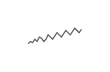
\begin{tikzpicture}[x=0.08em, y=0.08em, line width=0.4pt]
                \draw[FooterGray] (0,3) -- (1,4) -- (2,3.5) -- (3,5) -- (4,4) -- (5,6) -- (6,5.5) -- (7,4) -- (8,5) -- (9,7) -- (10,6) -- (11,5) -- (12,6.5) -- (13,8) -- (14,7) -- (15,6) -- (16,7.5) -- (17,9) -- (18,8) -- (19,7) -- (20,8.5) -- (21,10) -- (22,9) -- (23,8) -- (24,9.5);
            \end{tikzpicture}%
        }%
        \hskip0.5cm%
    }%
    \vskip6pt%
}

%=============================================================================
% PACKAGES
%=============================================================================
\usepackage[utf8]{inputenc}
\DeclareUnicodeCharacter{03B1}{\ensuremath{\alpha}}
\usepackage[T1]{fontenc}
\usepackage{amsmath, amssymb, amsthm}
\usepackage{mathtools}
\usepackage{bm}
\usepackage{tikz}
\usetikzlibrary{arrows.meta, positioning, shapes, calc, decorations.pathreplacing, shadings}
\usepackage{booktabs}
\usepackage{multirow}
\usepackage{array}
\usepackage{graphicx}
\usepackage{animate}
\usepackage{hyperref}
\usepackage{colortbl}
\usepackage{listings}
\lstset{language=Python, basicstyle=\ttfamily\scriptsize, keywordstyle=\color{MainBlue}\bfseries,
  commentstyle=\color{Forest}, stringstyle=\color{Crimson}, breaklines=true,
  frame=none, backgroundcolor=\color{VeryLightGray}, xleftmargin=2mm}
\hypersetup{colorlinks=true, linkcolor=MainBlue, urlcolor=MainBlue}
\graphicspath{{../../logos/}{../../charts/}{../../photos/}}
\usepackage{xcolor}
\hfuzz=2pt  % Suppress tiny overfull warnings (<2pt)
\vfuzz=2pt  % Suppress tiny vertical overfull warnings (<2pt)
% \mathrm in the sans-serif family of the slides (beamer resets \mathrm to the serif family at \begin{document};
% this hook runs after beamer's, so WN, Var, RMSE, ... in formulas match the surrounding text)
% Bold vectors and matrices in the same sans-serif family: \mathbf{A} in sans bold (beamer's own \mathbf came out in
% medium weight), and the bold upright Greek capitals of \boldsymbol / \bm (\bSigma, \bPhi, \boldsymbol{\Theta}) in
% cmss bold: bm.sty fixes its "boldoperators" font when it is loaded (serif cmbx), before beamer switches the
% operators to cmss, so it is reset here.
\AtBeginDocument{%
  \SetMathAlphabet{\mathrm}{normal}{\encodingdefault}{\sfdefault}{\mddefault}{n}%
  \SetMathAlphabet{\mathrm}{bold}{\encodingdefault}{\sfdefault}{bx}{n}%
  \SetMathAlphabet{\mathbf}{normal}{\encodingdefault}{\sfdefault}{bx}{n}%
  \SetMathAlphabet{\mathbf}{bold}{\encodingdefault}{\sfdefault}{bx}{n}%
  \SetSymbolFont{boldoperators}{normal}{OT1}{cmss}{bx}{n}%
  \SetSymbolFont{boldoperators}{bold}{OT1}{cmss}{bx}{n}}

%=============================================================================
% QUANTLET COMMANDS
%   \quantlet{<displayed name>}{<url>}       (generic, compatible with the older TSA decks)
%   \tsaquantlet{Ch_05}{TSA_ch5_garch}       -> https://github.com/danpele/Time-Series-Analysis/tree/main/Quantlets/Ch_05/TSA_ch5_garch
%   \qlurl{<folder>} is defined per chapter by the generator (Quantlets/Ch_NN/<folder>)
%=============================================================================
\newcommand{\tsarepo}{https://github.com/danpele/Time-Series-Analysis}
\newcommand{\tsaqlbase}{https://github.com/danpele/Time-Series-Analysis/tree/main/Quantlets}
\newcommand{\quantlet}[2]{%
    \hfill\href{#2}{%
        \raisebox{-0.15em}{
\includegraphics[height=0.7em]{ql_logo.png}}%
        \textcolor{MainBlue}{\tiny\ #1}%
    }%
}
\newcommand{\tsaquantlet}[2]{\quantlet{\detokenize{#2}}{\tsaqlbase/#1/#2}}

%=============================================================================
% NOTEBOOKS (Google Colab)
%   \colaburl{notebooks/EN/chapter5_seminar_notebook.ipynb} -> the Colab link of a file in the TSA repo
%   \nb: the chapter notebook (each seminar deck redefines it with \renewcommand)
%=============================================================================
\newcommand{\colaburl}[1]{https://colab.research.google.com/github/danpele/Time-Series-Analysis/blob/main/#1}
\newcommand{\nb}{https://colab.research.google.com/github/danpele/Time-Series-Analysis/tree/main/notebooks/EN}
\newcommand{\nbname}{notebooks/EN}

%=============================================================================
% SLIDE HELPERS (used by the generators; the same as in MFM)
%=============================================================================
% local font size for list bodies (the preamble forces \normalsize)
\newcommand{\itemsize}[1]{\setbeamertemplate{itemize/enumerate body begin}{#1}\setbeamertemplate{itemize/enumerate subbody begin}{#1}}
\newcommand{\intitle}[1]{{\hypersetup{urlcolor=white}#1}}   % white links inside coloured title bars
\newcommand{\imgcap}[1]{{\scriptsize #1}\\[0.5mm]}          % caption under a photo
\newcommand{\imgcredit}[2]{{\tiny\color{FooterGray}\href{#1}{#2}}}   % image credit: source URL, author/licence
\newcommand{\aiprompt}[1]{{\ttfamily\color{MainBlue}#1}}     % a prompt to an AI assistant

%=============================================================================
% SEMINARS: student version by default; the instructor wrapper *_solutions.tex sets \solutionstrue
%=============================================================================
\makeatletter\@ifundefined{ifsolutions}{\expandafter\newif\csname ifsolutions\endcsname}{}\makeatother
\newcommand{\solonly}[1]{\ifsolutions #1\fi}
\newcommand{\propsub}{\ifsolutions\else\framesubtitle{\ifdefined\tsalang Rezolvarea se discută la seminar\else Solution discussed in class\fi}\fi}

%=============================================================================
% APPENDIX AND CHAPTER LINKS (latex/appendix_links.py writes the calls; it also re-declares these
% macros before \begin{document}, so the decks compile with or without this preamble block)
%=============================================================================
\providecommand{\tsaapplink}[3]{\hypertarget{#2}{}\hyperlink{#1}{\beamergotobutton{#3}}}
\providecommand{\tsaappback}[2]{\begin{tikzpicture}[remember picture,overlay]\node[anchor=south east] at ([xshift=-3mm,yshift=7mm]current page.south east){\hyperlink{#1}{\beamerreturnbutton{#2}}};\end{tikzpicture}}
\providecommand{\tsachlink}[2]{\href{#1}{#2}}
\providecommand{\tsachlinkt}[2]{\href{#1}{\usebeamercolor[fg]{frametitle}#2}}

%=============================================================================
% QUANTINAR COMMAND: link către un curs Quantinar (subiecte avansate)
%=============================================================================
\newcommand{\quantinar}[2]{%
    \href{#2}{%
        \raisebox{-0.15em}{
\includegraphics[height=0.8em]{qr_logo.png}}%
        \textcolor{MainBlue}{\scriptsize\ #1}%
    }%
}

%=============================================================================
% CUSTOM TITLE PAGE
%=============================================================================
\defbeamertemplate*{title page}{hybrid}[1][]
{
    \vspace{0.2cm}
    % Logos row - top header (with clickable links)
    \begin{center}
        \href{https://www.ase.ro}{
\includegraphics[height=1.0cm]{ase_logo.png}}\hspace{0.3cm}%
        \href{https://theida.net}{
\includegraphics[height=1.0cm]{ida_logo.png}}\hspace{0.3cm}%
        \href{https://blockchain-research-center.com}{
\includegraphics[height=1.0cm]{brc_logo.png}}\hspace{0.3cm}%
        \href{https://www.ai4efin.ase.ro}{
\includegraphics[height=1.0cm]{ai4efin_logo.png}}\hspace{0.3cm}%
        \href{https://ipe.ro/new}{
\includegraphics[height=1.0cm]{acad_logo.png}}\hspace{0.3cm}%
        \href{https://www.digital-finance-msca.com}{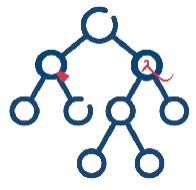
\includegraphics[height=1.0cm]{msca_logo.png}}%
    \end{center}

    \vspace{0.6cm}

    % Main title with Q logos on sides (with clickable links)
    \begin{center}
        \begin{minipage}{0.1\textwidth}
            \centering
            \href{https://quantlet.com}{
\includegraphics[height=1.1cm]{ql_logo.png}}
        \end{minipage}%
        \begin{minipage}{0.78\textwidth}
            \centering
            {\LARGE\bfseries\usebeamercolor[fg]{title}\inserttitle}

            \vspace{0.3cm}

            {\usebeamerfont{subtitle}\usebeamercolor[fg]{title}\insertsubtitle}
        \end{minipage}%
        \begin{minipage}{0.1\textwidth}
            \centering
            \href{https://quantinar.com}{
\includegraphics[height=1.1cm]{qr_logo.png}}
        \end{minipage}
    \end{center}

    \vspace{0.6cm}

    % Authors (left aligned)
    \hspace{0.5cm}{\usebeamerfont{author}\insertauthor}

    \vspace{0.3cm}

    % Institute/Affiliations (left aligned)
    \hspace{0.5cm}\begin{minipage}[t]{0.9\textwidth}
        \raggedright\small\insertinstitute
    \end{minipage}
}

%=============================================================================
% THEOREM ENVIRONMENTS
%=============================================================================
\theoremstyle{definition}
\setbeamertemplate{theorems}[numbered]
\ifdefined\tsalang
\newtheorem{defn}{Definiție}
\newtheorem{thm}{Teoremă}
\newtheorem{prop}{Propoziție}
\newtheorem{rmk}{Observație}
\else
\newtheorem{defn}{Definition}
\newtheorem{thm}{Theorem}
\newtheorem{prop}{Proposition}
\newtheorem{rmk}{Remark}
\fi

%=============================================================================
% CENTRED MINIPAGE (no extra vertical space)
%=============================================================================
\newenvironment{cminipage}[1]{%
    \par\noindent\hfill\begin{minipage}{#1}\ignorespaces
}{%
    \end{minipage}\hfill\null\par
}

%=============================================================================
% CUSTOM COMMANDS
%=============================================================================
\newcommand{\E}{\mathbb{E}}
\newcommand{\Var}{\text{Var}}
\newcommand{\Cov}{\text{Cov}}
\newcommand{\Corr}{\text{Corr}}
\newcommand{\R}{\mathbb{R}}
\newcommand{\N}{\mathbb{N}}
\newcommand{\Z}{\mathbb{Z}}
\newcommand{\B}{\mathbf{B}}
\newcommand{\imark}{\textcolor{MainBlue}{\textbullet}}
\newcommand{\RMSE}{\text{RMSE}}
\newcommand{\MAE}{\text{MAE}}
\newcommand{\MAPE}{\text{MAPE}}

% Boldface vector/matrix commands (VAR, VECM, state space; also used by the older TSA decks)
\newcommand{\bY}{\mathbf{Y}}
\newcommand{\bX}{\mathbf{X}}
\newcommand{\bA}{\mathbf{A}}
\newcommand{\bB}{\mathbf{B}}
\newcommand{\bepsilon}{\boldsymbol{\varepsilon}}
\newcommand{\bSigma}{\boldsymbol{\Sigma}}
\newcommand{\bPhi}{\boldsymbol{\Phi}}
\newcommand{\bGamma}{\boldsymbol{\Gamma}}
\newcommand{\bPi}{\boldsymbol{\Pi}}
\newcommand{\bc}{\mathbf{c}}
\newcommand{\balpha}{\boldsymbol{\alpha}}
\newcommand{\bbeta}{\boldsymbol{\beta}}
\newcommand{\bvarepsilon}{\boldsymbol{\varepsilon}}

% Legacy seminar marks (older TSA seminar decks)
\newcommand{\correct}{\textcolor{Forest}{\checkmark}}
\newcommand{\incorrect}{\textcolor{Crimson}{\texttimes}}


\newcommand{\qlurl}[1]{https://github.com/danpele/Time-Series-Analysis/tree/main/Quantlets/Ch_00/#1}

% Clickable citations (DOIs verified via Crossref)

\newcommand{\refHP}{\href{https://doi.org/10.1007/978-3-031-13584-2}{Huang \& Petukhina (2022)}}
\newcommand{\refFPP}{\href{https://otexts.com/fpp3/}{Hyndman \& Athanasopoulos (2021)}}
\newcommand{\refBD}{\href{https://doi.org/10.1007/978-3-319-29854-2}{Brockwell \& Davis (2016)}}
\newcommand{\refHamilton}{\href{https://doi.org/10.2307/j.ctv14jx6sm}{Hamilton (1994)}}
\newcommand{\refYuleNonsense}{\href{https://doi.org/10.2307/2341482}{Yule (1926)}}
\newcommand{\refYule}{\href{https://doi.org/10.1098/rsta.1927.0007}{Yule (1927)}}
\newcommand{\refSlutsky}{\href{https://doi.org/10.2307/1907241}{Slutzky (1937)}}
\newcommand{\refKolmogorov}{\href{https://doi.org/10.1007/978-94-011-2260-3_28}{Kolmogorov (1941)}}
\newcommand{\refWiener}{\href{https://doi.org/10.7551/mitpress/2946.001.0001}{Wiener (1949)}}
\newcommand{\refBJ}{\href{https://doi.org/10.1002/9781118619193}{Box \& Jenkins (1970)}}
\newcommand{\refHolt}{\href{https://doi.org/10.1016/j.ijforecast.2003.09.015}{Holt (1957)}}
\newcommand{\refWinters}{\href{https://doi.org/10.1287/mnsc.6.3.324}{Winters (1960)}}
\newcommand{\refGardner}{\href{https://doi.org/10.1002/for.3980040103}{Gardner (1985)}}
\newcommand{\refHKSG}{\href{https://doi.org/10.1016/S0169-2070(01)00110-8}{Hyndman, Koehler, Snyder \& Grose (2002)}}
\newcommand{\refHK}{\href{https://doi.org/10.1016/j.ijforecast.2006.03.001}{Hyndman \& Koehler (2006)}}
\newcommand{\refMthree}{\href{https://doi.org/10.1016/S0169-2070(00)00057-1}{Makridakis \& Hibon (2000)}}
\newcommand{\refMfour}{\href{https://doi.org/10.1016/j.ijforecast.2019.04.014}{Makridakis, Spiliotis \& Assimakopoulos (2020)}}
\newcommand{\refSTL}{\href{https://www.scb.se/contentassets/ca21efb41fee47d293bbee5bf7be7fb3/stl-a-seasonal-trend-decomposition-procedure-based-on-loess.pdf}{Cleveland et al.\ (1990)}}
\newcommand{\refKeeling}{\href{https://doi.org/10.3402/tellusa.v12i2.9366}{Keeling (1960)}}
\newcommand{\refEngle}{\href{https://doi.org/10.2307/1912773}{Engle (1982)}}
\newcommand{\refSims}{\href{https://doi.org/10.2307/1912017}{Sims (1980)}}
\newcommand{\refEG}{\href{https://doi.org/10.2307/1913236}{Engle \& Granger (1987)}}
\newcommand{\refStatsmodels}{\href{https://doi.org/10.25080/Majora-92bf1922-011}{Seabold \& Perktold (2010)}}
\newcommand{\refPandas}{\href{https://doi.org/10.25080/Majora-92bf1922-00a}{McKinney (2010)}}
\newcommand{\refNumpy}{\href{https://doi.org/10.1038/s41586-020-2649-2}{Harris et al.\ (2020)}}

\title[Time Series Analysis]{Time Series Analysis}
\subtitle{Chapter 0: Introduction: components and exponential smoothing}
\author[D.T. Pele]{Daniel Traian PELE}
\institute{Bucharest University of Economic Studies\\
IDA Institute Digital Assets\\
Blockchain Research Center\\
AI4EFin Artificial Intelligence for Energy Finance\\
Romanian Academy, Institute for Economic Forecasting\\
MSCA Digital Finance}
\date{}

%=============================================================================
\providecommand{\tsaapplink}[3]{\hypertarget{#2}{}\hyperlink{#1}{\beamergotobutton{#3}}}  % APPLINKS-MACROS
\providecommand{\tsaappback}[2]{\begin{tikzpicture}[remember picture,overlay]\node[anchor=south east] at ([xshift=-3mm,yshift=7mm]current page.south east){\hyperlink{#1}{\beamerreturnbutton{#2}}};\end{tikzpicture}}  % APPLINKS-MACROS
\providecommand{\tsachlink}[2]{\href{#1}{#2}}  % APPLINKS-MACROS
\providecommand{\tsachlinkt}[2]{\href{#1}{\usebeamercolor[fg]{frametitle}#2}}  % APPLINKS-MACROS
\begin{document}
%=============================================================================

{
\setbeamertemplate{headline}{}
\setbeamertemplate{footline}{}
\begin{frame}[noframenumbering]
    \titlepage
\end{frame}
}
% BEGIN-ACRONYMS (generat de latex/acronyms.py; nu editati manual)
\begin{frame}{Acronyms used in this material (1/2)}
\setbeamertemplate{itemize/enumerate body begin}{\tiny}
\begin{columns}[T]
\begin{column}{0.49\textwidth}
\begin{itemize}\setlength{\itemsep}{0pt}
    \item \textbf{ACF}: Autocorrelation Function
    \item \textbf{AI}: Artificial Intelligence
    \item \textbf{API}: Application Programming Interface
    \item \textbf{AR}: AutoRegressive (model); in event studies: Abnormal Return
    \item \textbf{ARCH}: AutoRegressive Conditional Heteroskedasticity
    \item \textbf{ARFIMA}: AutoRegressive Fractionally Integrated Moving Average (model)
    \item \textbf{ARIMA}: AutoRegressive Integrated Moving Average (model)
    \item \textbf{ARMA}: AutoRegressive Moving Average (model)
    \item \textbf{ASE}: Academia de Studii Economice din București (the Bucharest University of Economic Studies)
    \item \textbf{BET}: Bucharest Exchange Trading (index)
    \item \textbf{BNR}: Banca Națională a României (the National Bank of Romania)
    \item \textbf{BVB}: Bursa de Valori București (the Bucharest Stock Exchange)
    \item \textbf{CO2}: Carbon dioxide
\end{itemize}
\end{column}
\begin{column}{0.49\textwidth}
\begin{itemize}\setlength{\itemsep}{0pt}
    \item \textbf{COVID-19}: COronaVIrus Disease 2019
    \item \textbf{CSIE}: Facultatea de Cibernetică, Statistică și Informatică Economică (the Faculty of Cybernetics, Statistics and Economic Informatics)
    \item \textbf{ECTS}: European Credit Transfer and Accumulation System
    \item \textbf{EOD}: End Of Day (daily closing data)
    \item \textbf{EODHD}: EOD Historical Data (market-data provider)
    \item \textbf{ETS}: Error, Trend, Seasonality (exponential smoothing state space models)
    \item \textbf{EU}: European Union
    \item \textbf{FRED}: Federal Reserve Economic Data
    \item \textbf{GARCH}: Generalised AutoRegressive Conditional Heteroskedasticity
    \item \textbf{GDP}: Gross Domestic Product
    \item \textbf{HICP}: Harmonised Index of Consumer Prices
    \item \textbf{INS}: Institutul Național de Statistică (the National Institute of Statistics (Romania))
    \item \textbf{LLM}: Large Language Model
\end{itemize}
\end{column}
\end{columns}
\end{frame}
\begin{frame}{Acronyms used in this material (2/2)}
\setbeamertemplate{itemize/enumerate body begin}{\tiny}
\begin{columns}[T]
\begin{column}{0.49\textwidth}
\begin{itemize}\setlength{\itemsep}{0pt}
    \item \textbf{LOESS}: LOcally Estimated Scatterplot Smoothing
    \item \textbf{LPPL}: Log-Periodic Power Law
    \item \textbf{MA}: Moving Average
    \item \textbf{MAE}: Mean Absolute Error
    \item \textbf{MAPE}: Mean Absolute Percentage Error
    \item \textbf{MASE}: Mean Absolute Scaled Error
    \item \textbf{RMSE}: Root Mean Squared Error
    \item \textbf{SARIMA}: Seasonal ARIMA (model)
    \item \textbf{SES}: Simple Exponential Smoothing
    \item \textbf{STL}: Seasonal and Trend decomposition using Loess
    \item \textbf{TBATS}: Trigonometric seasonality, Box–Cox, ARMA errors, Trend, Seasonal components (model)
    \item \textbf{TRAMO-SEATS}: Time series Regression with ARIMA noise, Missing values and Outliers; Signal Extraction in ARIMA Time Series
    \item \textbf{US}: United States
\end{itemize}
\end{column}
\begin{column}{0.49\textwidth}
\begin{itemize}\setlength{\itemsep}{0pt}
    \item \textbf{VAR}: Vector AutoRegression
    \item \textbf{VAT}: Value Added Tax
    \item \textbf{VECM}: Vector Error Correction Model
\end{itemize}
\end{column}
\end{columns}
\end{frame}
% END-ACRONYMS

%=============================================================================
\section{Course Organisation}
%=============================================================================

\begin{frame}{Route of This Chapter}
\itemsize{\footnotesize}
\begin{columns}[T]
\begin{column}{0.47\textwidth}
\begin{itemize}
    \item \textbf{Guiding questions}
    \begin{itemize}
        \item what is a time series, and where do we meet one?
        \item which patterns repeat in economic, financial, energy and climate data?
        \item how do we forecast a series, and how do we know the forecast is good?
    \end{itemize}
    \item \textbf{Part I}
    \begin{itemize}
        \item how the course works
        \item time series on real data and a short history
        \item components: trend, seasonality, cycle, noise
    \end{itemize}
    \item \textbf{Part II}
    \begin{itemize}
        \item notation, transformations and a first look at the ACF
        \item exponential smoothing; forecasts and their evaluation
        \item tools, and the possible contribution of AI
    \end{itemize}
\end{itemize}
\end{column}
\begin{column}{0.50\textwidth}
\begin{itemize}
    \item \textbf{Learning outcomes}: after this chapter you can
    \begin{itemize}
        \item explain how the course is organised and graded
        \item recognise trend, seasonality, cycle and noise in a chart
        \item compute growth rates, a moving average and a sample autocorrelation
        \item produce naive and exponential smoothing forecasts
        \item evaluate forecasts on a test set with MAE, RMSE and MASE
    \end{itemize}
    \item Seminar 0 comes \textbf{before} this lecture and practises the first tools on data
\end{itemize}
\end{column}
\end{columns}
\end{frame}

\begin{frame}{The Course at a Glance}
\itemsize{\footnotesize}
\begin{columns}[T]
\begin{column}{0.56\textwidth}
\begin{itemize}
    \item \textbf{Programme}
    \begin{itemize}
        \item Bachelor's programmes Economic Informatics and Economic Cybernetics, year 3, semester 2
        \item Faculty of Cybernetics, Statistics and Economic Informatics (CSIE), ASE Bucharest
        \item 4 ECTS credits; 2 hours of lecture and 1 hour of seminar a week; academic year 2026/2027
    \end{itemize}
    \item \textbf{Lecture}
    \begin{itemize}
        \item Prof.\ Daniel Traian Pele, \href{mailto:danpele@ase.ro}{danpele@ase.ro}
    \end{itemize}
    \item \textbf{Prerequisites}
    \begin{itemize}
        \item probability and statistics, econometrics (linear regression), Python
    \end{itemize}
    \item \textbf{Course website}
    \begin{itemize}
        \item \href{https://danpele.github.io/Time-Series-Analysis/}{danpele.github.io/Time-Series-Analysis}: slides, seminars, notebooks, Quantlets, quizzes
    \end{itemize}
\end{itemize}
\end{column}
\begin{column}{0.40\textwidth}
\centering
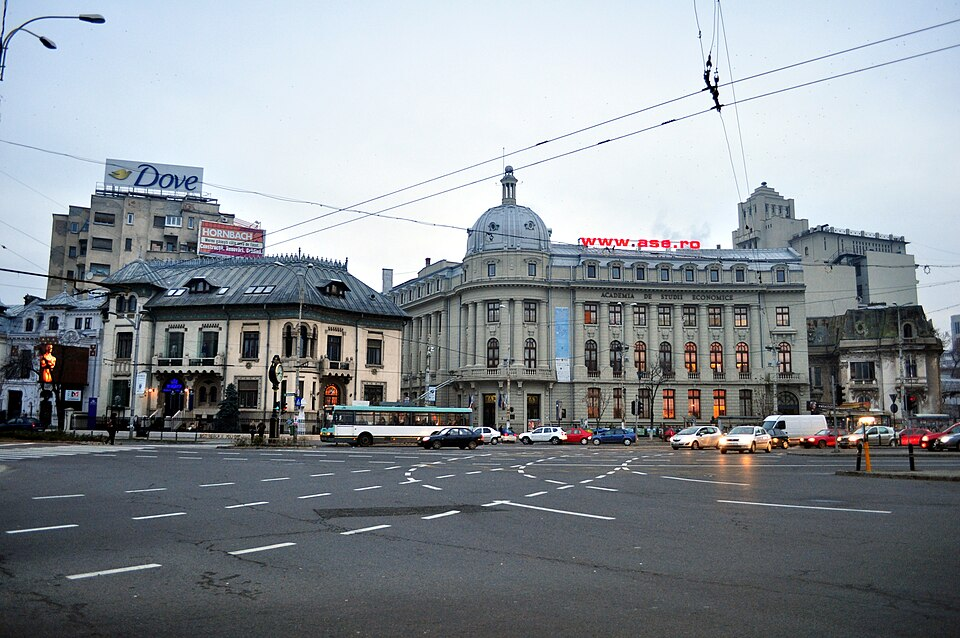
\includegraphics[height=0.46\textheight]{ch0_ase_2014.jpg}\\[1mm]
\imgcap{The Bucharest University of Economic Studies (ASE)}
\imgcredit{https://commons.wikimedia.org/wiki/File:Bucharest_-_Academie_de_Studii_Economice_01.jpg}{Photo: Joe Mabel (2014); CC BY 3.0; Wikimedia Commons}
\end{column}
\end{columns}
\end{frame}

\begin{frame}{Evaluation}
\itemsize{\small}
\begin{itemize}
    \item \textbf{Written exam: 70\%}
    \begin{itemize}
        \item reading and interpreting software output, short derivations, choosing a model for a given series
        \item covers the lectures and seminars of \tsachlink{https://danpele.github.io/Time-Series-Analysis/EN/Courses/chapter0_introduction.pdf}{Chapters 0}--10 and 15
    \end{itemize}
    \item \textbf{Team project: 20\%}
    \begin{itemize}
        \item 2--4 students analyse and forecast real time series with the methods of the course
        \item a GitHub repository, a short report, a presentation and an oral defence
    \end{itemize}
    \item \textbf{Attendance: 10\%}
    \begin{itemize}
        \item lectures and seminars
    \end{itemize}
    \item \textbf{Self-assessment quizzes}
    \begin{itemize}
        \item one per chapter on the website: 20 questions drawn from a bank of 24, each answer explained
    \end{itemize}
\end{itemize}
\end{frame}

\begin{frame}{Textbooks}
\itemsize{\small}
\begin{itemize}
    \item \textbf{Main textbook}
    \begin{itemize}
        \item \refHP, \emph{Applied Time Series Analysis and Forecasting with Python}, Springer
        \item the chapters of the course follow its order: components and smoothing, stationarity, ARMA, ARIMA, seasonality, volatility, multivariate models
    \end{itemize}
    \item \textbf{Free companion}
    \begin{itemize}
        \item \refFPP, \emph{Forecasting: Principles and Practice} (3rd edition, online)
        \item the reference for decomposition, exponential smoothing and forecast evaluation (\tsachlink{https://danpele.github.io/Time-Series-Analysis/EN/Courses/chapter0_introduction.pdf}{Chapter 0})
    \end{itemize}
    \item \textbf{Theory}
    \begin{itemize}
        \item \refBD, \emph{Introduction to Time Series and Forecasting}
        \item \refHamilton, \emph{Time Series Analysis}: the standard reference of time series econometrics
    \end{itemize}
\end{itemize}
\end{frame}

\begin{frame}{Course Map: \tsachlinkt{https://danpele.github.io/Time-Series-Analysis/EN/Courses/chapter0_introduction.pdf}{Chapters 0}--15}
\itemsize{\footnotesize}
\begin{columns}[T]
\begin{column}{0.49\textwidth}
\begin{center}
\scriptsize
\begin{tabular}{r>{\raggedright\arraybackslash}p{6.2cm}}
\toprule
\textbf{No.} & \textbf{Chapter} \\
\midrule
0 & Introduction: components and exponential smoothing \\
1 & Stochastic processes and stationarity \\
2 & ARMA models \\
3 & Unit roots and ARIMA models \\
4 & Seasonality and forecasting: SARIMA, TBATS, Prophet \\
5 & Conditional volatility: ARCH and GARCH \\
6 & VAR models and Granger causality \\
7 & Cointegration and VECM \\
\bottomrule
\end{tabular}
\end{center}

\end{column}
\begin{column}{0.49\textwidth}
\begin{center}
\scriptsize
\begin{tabular}{r>{\raggedright\arraybackslash}p{6.2cm}}
\toprule
\textbf{No.} & \textbf{Chapter} \\
\midrule
8 & Long memory and ARFIMA \\
9 & Machine learning for time series \\
10 & State space models, Kalman filter and Markov switching \\
11 & Foundation models for time series$^*$ \\
12 & Spectral analysis$^*$ \\
13 & Speculative bubbles: LPPL models$^*$ \\
14 & Multivariate GARCH models$^*$ \\
15 & Review and exam preparation \\
\bottomrule
\end{tabular}
\end{center}

\end{column}
\end{columns}
\begin{itemize}
    \item Univariate models (0--5), several series (6, 7), extensions (8--10), review (15)
    \item $^*$ Chapters 11--14: self-study (shorter materials and a quiz, no compulsory seminar)
\end{itemize}
\end{frame}

\begin{frame}{Materials and Tools}
\itemsize{\small}
\begin{itemize}
    \item \textbf{For every chapter}
    \begin{itemize}
        \item lecture and seminar slides, in Romanian and in English
        \item a lecture notebook and a seminar notebook (Python), opened in Google Colab with one click
        \item a quiz of 20 questions
    \end{itemize}
    \item \textbf{Quantlets}: every chart has a public folder with its code, a description file (\texttt{Metainfo.txt}) and the chart
    \begin{itemize}
        \item the icon under each chart opens its Quantlet on GitHub
    \end{itemize}
    \item \textbf{Data}: public sources, read directly in the code
    \begin{itemize}
        \item Eurostat, INS (National Institute of Statistics), BNR (National Bank of Romania), FRED (Federal Reserve Bank of St.\ Louis)
        \item daily market data from EODHD (EOD Historical Data), saved in the course repository until 18 September 2026
    \end{itemize}
\end{itemize}
\end{frame}

\begin{frame}{Seminars}
\itemsize{\small}
\begin{itemize}
    \item \textbf{Each seminar comes before its lecture}
    \begin{itemize}
        \item it starts with a short primer, so it can be followed without the lecture
        \item the lecture then explains why the tools work and where they fail
    \end{itemize}
    \item \textbf{Three parts}
    \begin{itemize}
        \item A: short calculations on paper; B: real data, each task ending with an interpretation question; C: an open idea and the critique of an AI answer
    \end{itemize}
    \item \textbf{Two kinds of exercises}
    \begin{itemize}
        \item \textbf{[Solved]}: full solution in the slides and in the notebook, a model to follow
        \item \textbf{[Proposed]}: you solve it; the solution is discussed in class
    \end{itemize}
    \item \textbf{Nothing is handed in}: the seminar is practice for the exam and for the project
\end{itemize}
\end{frame}

\begin{frame}{The Team Project}
\itemsize{\small}
\begin{itemize}
    \item \textbf{Question}: one forecasting or modelling question on real time series, chosen by the team
    \item \textbf{Methods}: those of the course
    \begin{itemize}
        \item decomposition and smoothing, ARIMA and SARIMA, GARCH, VAR or VECM, Granger causality, impulse responses, forecast evaluation
        \item Romanian data (INS, BNR, Eurostat, BVB) are encouraged
    \end{itemize}
    \item \textbf{Deliverables}
    \begin{itemize}
        \item a GitHub repository whose code reproduces every number and every chart
        \item a short report, a presentation and the file \texttt{AI\_USE.md}
    \end{itemize}
    \item \textbf{Grading}
    \begin{itemize}
        \item a clear question, correct methods and diagnostics, an honest out-of-sample evaluation
        \item \textbf{oral defence}: each member explains the code and the results
    \end{itemize}
\end{itemize}
\end{frame}

\begin{frame}{AI Policy}
\itemsize{\small}
\begin{itemize}
    \item \textbf{AI tools are allowed and must be declared}
    \begin{itemize}
        \item AI: artificial intelligence; here, assistants based on an LLM (large language model) that write text and code
        \item every use goes into \texttt{AI\_USE.md}: the tool, the prompt, what was kept, what was corrected
    \end{itemize}
    \item \textbf{You are responsible for every number and every reference}
    \begin{itemize}
        \item typical AI errors: invented references, wrong formulas, code that runs but computes something else
        \item every reference: open its DOI (Digital Object Identifier) and check the title
        \item every number: recompute it with your own code
    \end{itemize}
    \item \textbf{Oral defence}
    \begin{itemize}
        \item a line of code you cannot explain does not count as your work
    \end{itemize}
\end{itemize}
\end{frame}

\begin{frame}{Recap: Organisation}
\itemsize{\small}
\begin{itemize}
    \item Grade: 70\% written exam, 20\% team project, 10\% attendance
    \item Textbook: \refHP; free companion: \refFPP
    \item \tsachlink{https://danpele.github.io/Time-Series-Analysis/EN/Courses/chapter0_introduction.pdf}{Chapters 0}--15; Chapters 11--14 are self-study
    \item Seminars come before lectures; nothing is handed in
    \item AI is allowed, declared in \texttt{AI\_USE.md}, and checked at the oral defence
\end{itemize}
\end{frame}


%=============================================================================
\section{What a Time Series Is}
%=============================================================================

\begin{frame}{Definition}
\itemsize{\small}
\begin{itemize}
    \item \textbf{Time series}: observations of one variable, recorded at successive moments and ordered in time
    \item \textbf{Notation}: $y_1, y_2, \ldots, y_T$
    \begin{itemize}
        \item $t$: the time index (quarter, month, day); $T$: the number of observations
        \item \textbf{frequency}: the number of observations per year (4 quarterly, 12 monthly, about 252 for trading days)
    \end{itemize}
    \item \textbf{Example}: Romanian real GDP, quarterly, billion EUR at 2010 prices
    \begin{itemize}
        \item 2024 Q1: 38.7; 2024 Q2: 45.6; 2024 Q3: 52.8; 2024 Q4: 59.2; 2025 Q1: 38.9
        \item the order matters: shuffling the five numbers destroys the information
    \end{itemize}
    \item GDP: gross domestic product; Q1--Q4: the four quarters of a year
\end{itemize}
\end{frame}

\begin{frame}{Three Kinds of Data}
\itemsize{\footnotesize}
\begin{center}
\footnotesize
\begin{tabular}{>{\raggedright\arraybackslash}p{2.6cm}>{\raggedright\arraybackslash}p{4.2cm}>{\raggedright\arraybackslash}p{5.4cm}}
\toprule
\textbf{Type} & \textbf{Structure} & \textbf{Example} \\
\midrule
Cross-section & many units, one moment & GDP of the 27 EU countries in 2025 \\
Time series & one unit, many moments & Romanian GDP, every quarter since 1995 \\
Panel & many units, many moments & GDP of the 27 EU countries, every quarter \\
\bottomrule
\end{tabular}
\end{center}
\begin{itemize}
    \item \textbf{What changes in a time series}
    \begin{itemize}
        \item observations are \textbf{not independent}: this quarter resembles the previous one
        \item this dependence is the information we use to forecast
        \item the classical formulas for independent samples (standard errors, tests) must be adapted
    \end{itemize}
    \item EU: European Union
\end{itemize}
\end{frame}

\begin{frame}{Why Time Series Matter}
\itemsize{\footnotesize}
\begin{center}
\footnotesize
\begin{tabular}{>{\raggedright\arraybackslash}p{1.9cm}>{\raggedright\arraybackslash}p{4.3cm}>{\raggedright\arraybackslash}p{6.2cm}}
\toprule
\textbf{Field} & \textbf{Series} & \textbf{Typical question} \\
\midrule
Economics & GDP, inflation, unemployment & Where will inflation be in a year? \\
Finance & exchange rates, stock indices, interest rates & How risky is the BET tomorrow? \\
Energy & electricity production and consumption, prices & How much electricity is needed next January? \\
Climate & CO2 concentration, temperatures & How fast does CO2 rise, beyond the seasonal swing? \\
\bottomrule
\end{tabular}
\end{center}
\begin{itemize}
    \item Decisions depend on forecasts: the central bank sets the interest rate on its inflation forecast; the grid operator plans production on its demand forecast
\end{itemize}
\end{frame}

\begin{frame}{Four Goals of Time Series Analysis}
\itemsize{\small}
\begin{itemize}
    \item \textbf{Describe}: trend, seasonality, cycles, unusual observations
    \begin{itemize}
        \item charts, decomposition, autocorrelation (this chapter and \tsachlink{https://danpele.github.io/Time-Series-Analysis/EN/Courses/chapter1_stochastic_processes_stationarity.pdf}{Chapter 1})
    \end{itemize}
    \item \textbf{Model}: a probability model that could have produced the data
    \begin{itemize}
        \item ARMA, ARIMA, GARCH (Chapters 2--5)
    \end{itemize}
    \item \textbf{Forecast}: values not yet observed, with their uncertainty
    \begin{itemize}
        \item the goal that runs through the whole course
    \end{itemize}
    \item \textbf{Explain and control}: how one series responds to another
    \begin{itemize}
        \item VAR models, Granger causality, cointegration (Chapters 6 and 7)
    \end{itemize}
    \item \refBJ\ framed the same goals: identify, estimate, check, forecast
\end{itemize}
\end{frame}

\begin{frame}{Frequency, Flows and Stocks, Adjusted Data}
\itemsize{\small}
\begin{itemize}
    \item \textbf{Flow}: measured over a period; \textbf{stock}: measured at a moment
    \begin{itemize}
        \item flows: GDP of a quarter, electricity produced in a month; they add up over time
        \item stocks: exchange rate on a day, CO2 concentration, an index level; we average them, we do not add them
    \end{itemize}
    \item \textbf{Changing the frequency}
    \begin{itemize}
        \item monthly to quarterly: the sum for flows, the average or the last value for stocks
    \end{itemize}
    \item \textbf{Seasonally adjusted data}
    \begin{itemize}
        \item the statistical office removes the regular within-year pattern and the calendar effects (number of working days)
        \item the unadjusted series is what was measured; the adjusted one is an estimate, revised when new data arrive
    \end{itemize}
\end{itemize}
\end{frame}

\begin{frame}{Data Used in This Chapter}
\itemsize{\footnotesize}
\begin{center}
\footnotesize
\begin{tabular}{>{\raggedright\arraybackslash}p{4.0cm}>{\raggedright\arraybackslash}p{3.0cm}>{\raggedright\arraybackslash}p{2.6cm}>{\raggedright\arraybackslash}p{2.8cm}}
\toprule
\textbf{Series} & \textbf{Source} & \textbf{Frequency} & \textbf{Sample} \\
\midrule
Romanian real GDP & Eurostat & quarterly & 1995 Q1 -- 2026 Q2 \\
Romanian HICP (consumer prices) & Eurostat & monthly & 1996 -- August 2026 \\
Electricity generation, Romania & Eurostat & monthly & January 2008 -- July 2026 \\
EUR/RON & BNR reference rate & daily & 2005 -- 2026 \\
BET, S\&P 500 & EODHD & daily & 2000 -- 2026 \\
CO2 at Mauna Loa & statsmodels data set & weekly, averaged monthly & 1958 -- 2001 \\
\bottomrule
\end{tabular}
\end{center}
\begin{itemize}
    \item HICP: Harmonised Index of Consumer Prices, computed with the same method in every EU country
    \item BET: the reference index of the BVB (Bucharest Stock Exchange); S\&P 500: 500 large US companies
    \item statsmodels: the Python library for statistical models used throughout the course
\end{itemize}
\end{frame}

\begin{frame}{Recap: What a time series is}
\itemsize{\small}
\begin{itemize}
    \item A time series is one variable observed over time; the order of the observations carries information
    \item Consecutive observations depend on each other: this is the basis of forecasting
    \item Goals: describe, model, forecast, explain
    \item Flows add up, stocks are averaged; adjusted series are estimates
\end{itemize}
\end{frame}


%=============================================================================
\section{Time Series on Real Data}
%=============================================================================

\begin{frame}{Romanian Real GDP}
\itemsize{\footnotesize}
\begin{center}
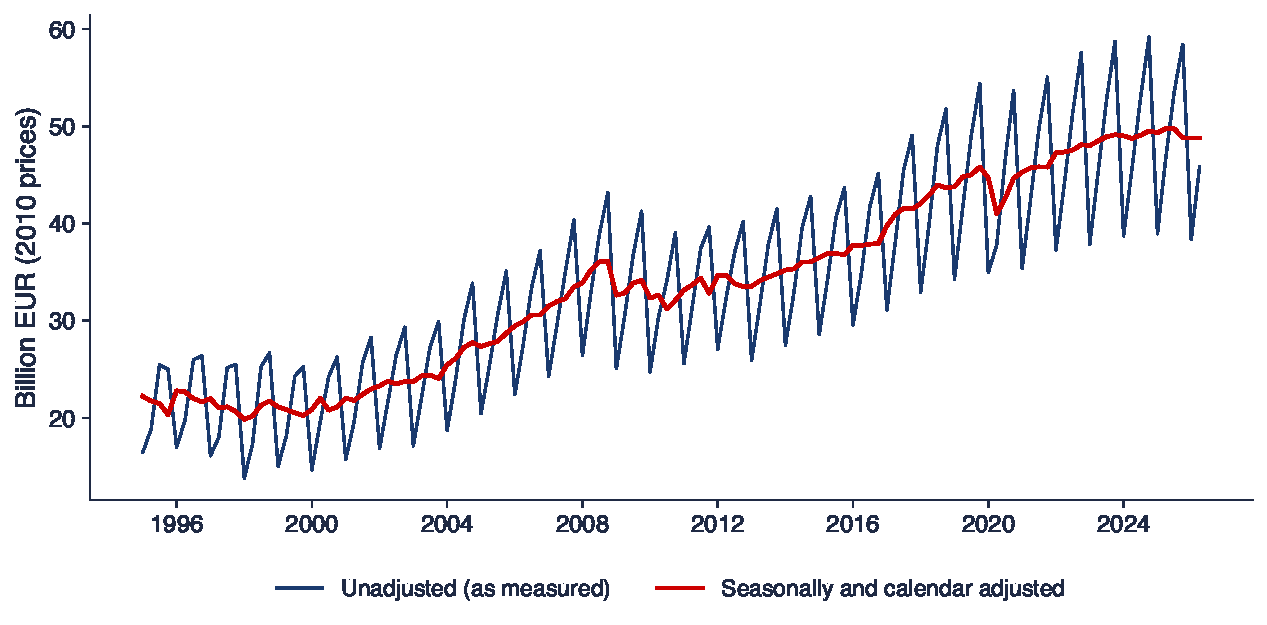
\includegraphics[width=0.94\textwidth,height=0.6\textheight,keepaspectratio]{tsa_ch0_gdp.pdf}
\end{center}
\vspace{-2mm}
\begin{itemize}
    \item Quarterly, 1995 Q1 -- 2026 Q2, chain-linked volumes at 2010 prices (billion EUR); blue: as measured; red: seasonally and calendar adjusted (Eurostat)
\end{itemize}
\quantlet{TSA\_ch0\_examples}{\qlurl{TSA_ch0_examples}}
\end{frame}

\begin{frame}{Interpretation: GDP}
\itemsize{\small}
\begin{itemize}
    \item \textbf{Trend}: the economy grew about 2.3 times from 1995 to 2025
    \begin{itemize}
        \item an average real growth of 2.8\% a year
    \end{itemize}
    \item \textbf{Seasonality}: every year, Q1 is far below Q4
    \begin{itemize}
        \item winter: less construction and agriculture; autumn: the harvest and year-end activity
        \item the swing grows with the level of GDP: a multiplicative pattern
    \end{itemize}
    \item \textbf{Cycle}: recessions interrupt the trend
    \begin{itemize}
        \item annual GDP fell by 5.5\% in 2009 (global financial crisis) and by 3.6\% in 2020 (COVID-19 pandemic)
    \end{itemize}
    \item Last value, 2026 Q2: 45.9 billion EUR unadjusted, 48.8 adjusted
\end{itemize}
\end{frame}

\begin{frame}{Romanian Consumer Prices and Inflation}
\itemsize{\footnotesize}
\begin{center}
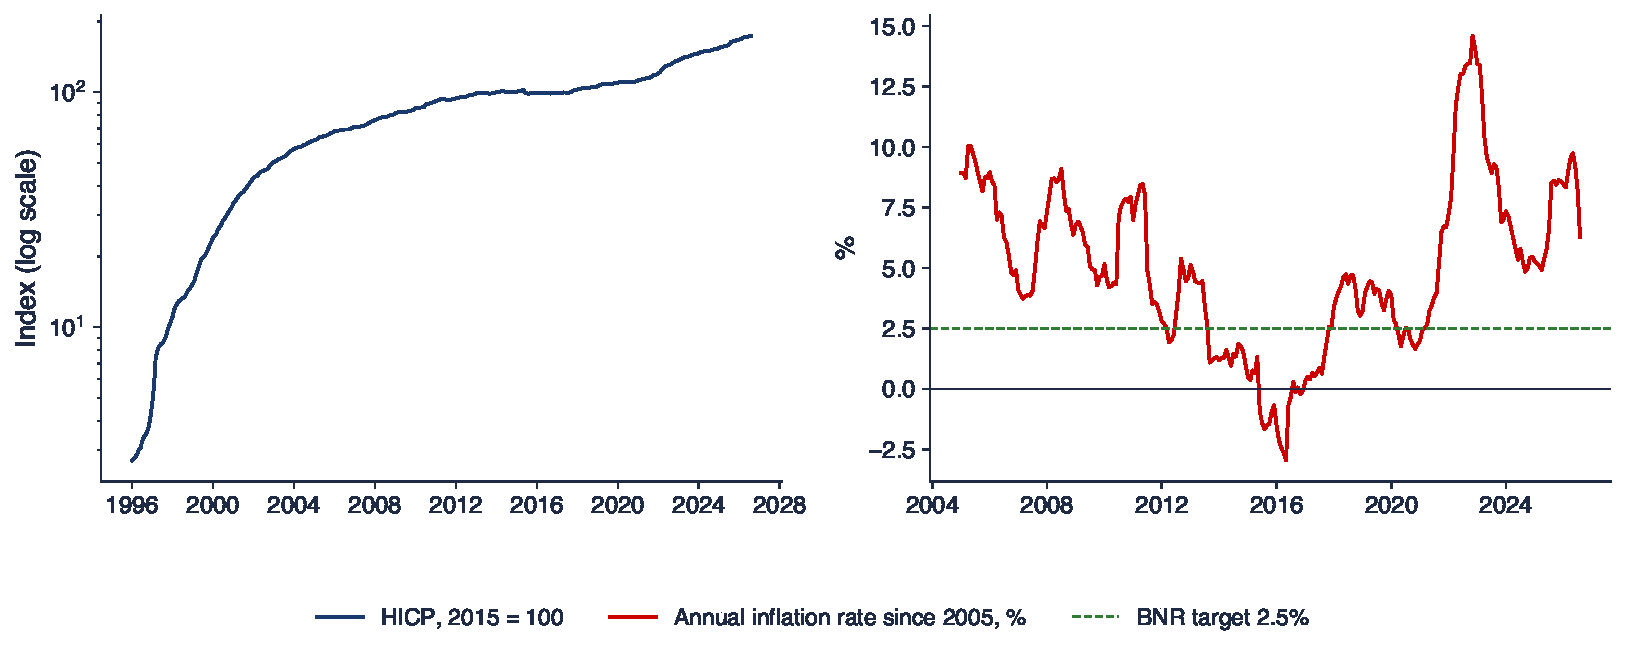
\includegraphics[width=0.94\textwidth,height=0.58\textheight,keepaspectratio]{tsa_ch0_hicp.pdf}
\end{center}
\vspace{-2mm}
\begin{itemize}
    \item Left: HICP, 2015 = 100, log scale; right: annual inflation rate $100\,(P_t/P_{t-12} - 1)$ since 2005, against the BNR target of 2.5\%
\end{itemize}
\quantlet{TSA\_ch0\_examples}{\qlurl{TSA_ch0_examples}}
\end{frame}

\begin{frame}{Interpretation: Inflation}
\itemsize{\small}
\begin{itemize}
    \item \textbf{Level and rate tell different stories}
    \begin{itemize}
        \item the price index almost never falls: its trend is the accumulated inflation
        \item the inflation rate rises and falls: it is the series the central bank targets
    \end{itemize}
    \item \textbf{Episodes}
    \begin{itemize}
        \item June 1997: 178\%, after the price liberalisation of 1997
        \item May 2016: -3.0\%, after the VAT cuts of 2015--2016
        \item November 2022: 14.6\%, the energy price shock
        \item August 2026: 6.3\%
    \end{itemize}
    \item A rate over 12 months removes the seasonal pattern but reacts with a delay: it reflects the whole past year
    \item VAT: value added tax
\end{itemize}
\end{frame}

\begin{frame}{EUR/RON, BNR Reference Rate}
\itemsize{\footnotesize}
\begin{center}
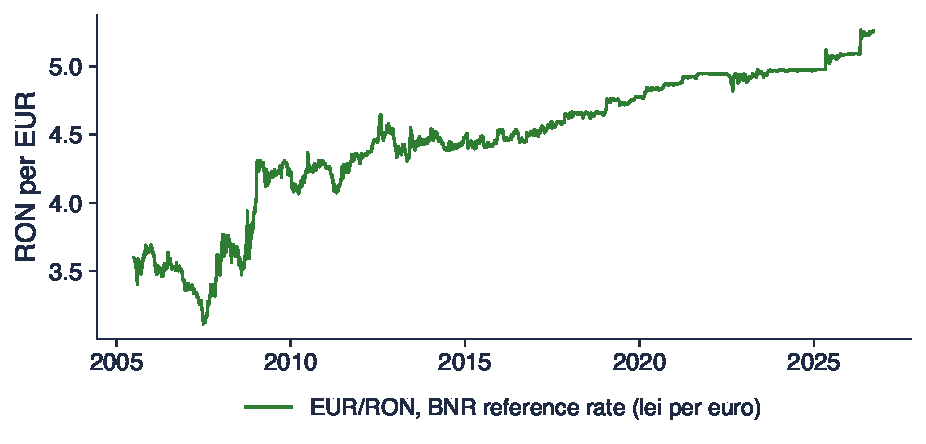
\includegraphics[width=0.94\textwidth,height=0.6\textheight,keepaspectratio]{tsa_ch0_eurron.pdf}
\end{center}
\vspace{-2mm}
\begin{itemize}
    \item Lei per euro, every working day from 4 July 2005 to 18 September 2026 (5\,353 observations)
\end{itemize}
\quantlet{TSA\_ch0\_examples}{\qlurl{TSA_ch0_examples}}
\end{frame}

\begin{frame}{Interpretation: EUR/RON}
\itemsize{\small}
\begin{itemize}
    \item \textbf{A trend without a fixed shape}
    \begin{itemize}
        \item from 3.5986 to 5.2644 lei; lowest value 3.1112 on 2 July 2007
        \item long calm periods, interrupted by jumps (autumn 2008, 2012, 2025)
    \end{itemize}
    \item \textbf{No seasonality}
    \begin{itemize}
        \item if the euro were predictably cheaper every spring, traders would buy it in spring and the pattern would disappear
    \end{itemize}
    \item \textbf{Daily changes}
    \begin{itemize}
        \item standard deviation of the daily log change: 0.28\%; the largest move: 2.93\% on 3 October 2008
    \end{itemize}
    \item A trend like this one, built from accumulated shocks, is called a \textbf{stochastic trend} (\tsachlink{https://danpele.github.io/Time-Series-Analysis/EN/Courses/chapter1_stochastic_processes_stationarity.pdf}{Chapters 1} and 3)
\end{itemize}
\end{frame}

\begin{frame}{BET and S\&P 500 since 2000}
\itemsize{\footnotesize}
\begin{center}
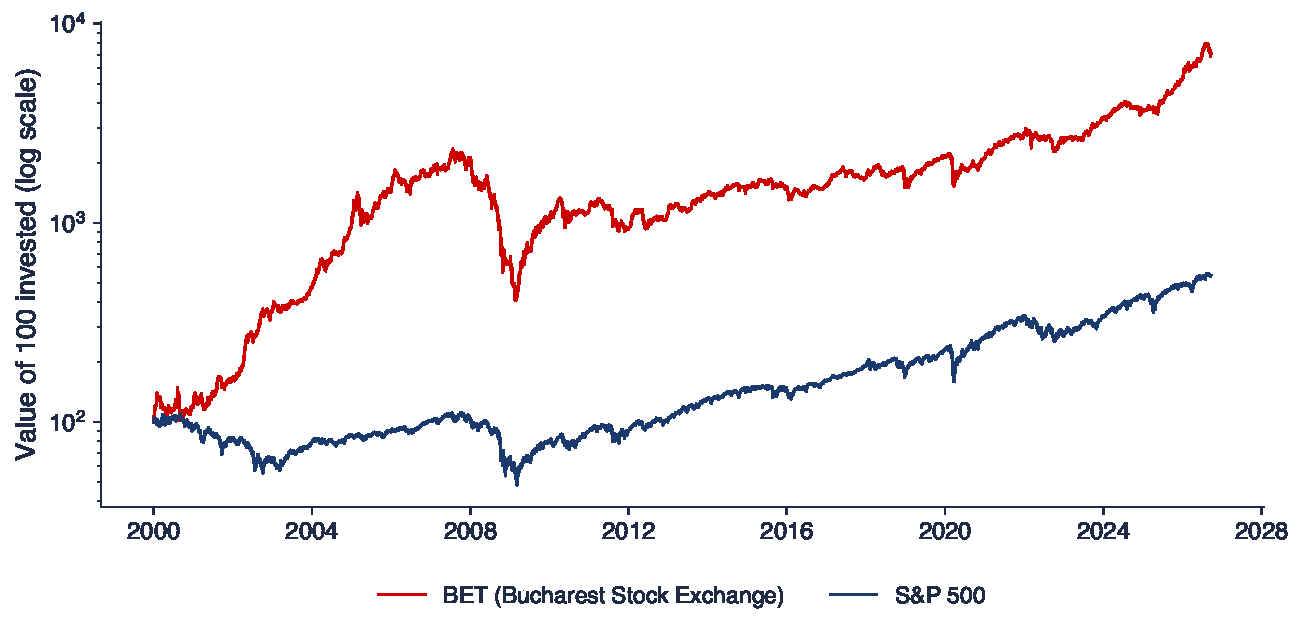
\includegraphics[width=0.94\textwidth,height=0.6\textheight,keepaspectratio]{tsa_ch0_markets.pdf}
\end{center}
\vspace{-2mm}
\begin{itemize}
    \item Value of 100 invested on 5 January 2000, closing prices, log scale: equal vertical distances are equal percentage changes
\end{itemize}
\quantlet{TSA\_ch0\_examples}{\qlurl{TSA_ch0_examples}}
\end{frame}

\begin{frame}{Interpretation: Stock Indices}
\itemsize{\small}
\begin{itemize}
    \item \textbf{Long-run growth with deep falls}
    \begin{itemize}
        \item 100 invested became about 71 times more in the BET and 5.5 times more in the S\&P 500 (price indices, without dividends)
        \item 2008--2009: the BET lost more than three quarters of its value; it took years to recover
    \end{itemize}
    \item \textbf{Why the log scale}
    \begin{itemize}
        \item on a linear scale, the early years look flat and recent moves look huge
        \item the logarithm turns constant percentage growth into a straight line
    \end{itemize}
    \item Prices of traded assets are hard to forecast; their \textbf{risk} is easier to forecast (Chapter 5)
\end{itemize}
\end{frame}

\begin{frame}{Electricity Generation in Romania}
\itemsize{\footnotesize}
\begin{center}
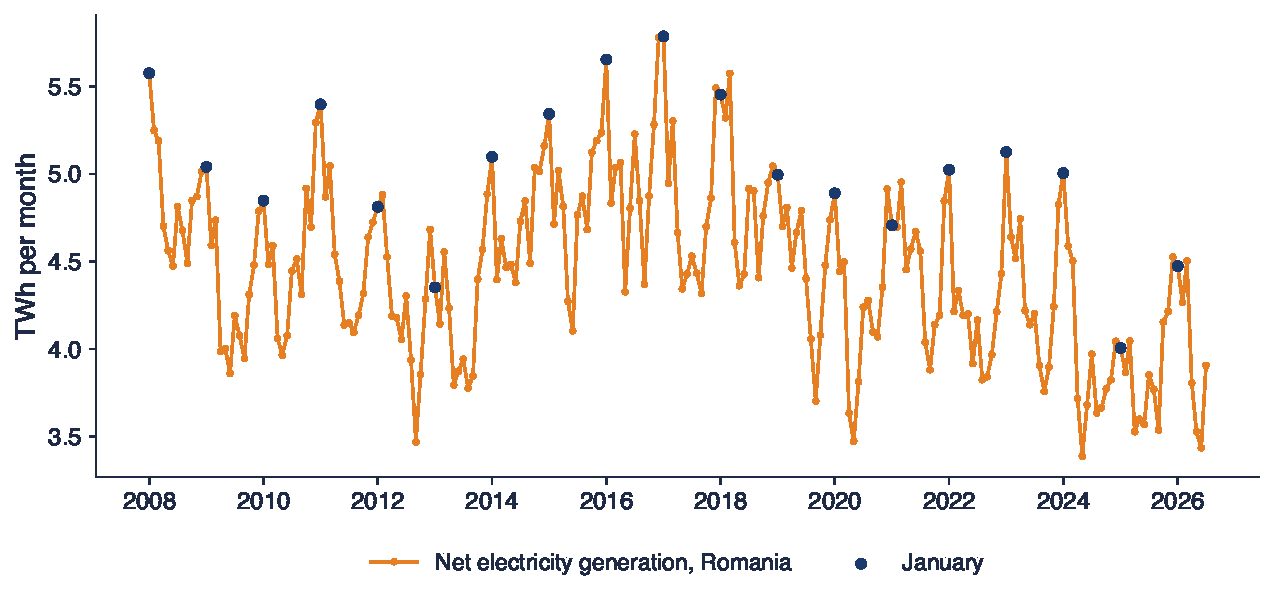
\includegraphics[width=0.94\textwidth,height=0.58\textheight,keepaspectratio]{tsa_ch0_electricity.pdf}
\end{center}
\vspace{-2mm}
\begin{itemize}
    \item Net electricity generation, TWh per month, January 2008 -- July 2026 (Eurostat); dots: January of each year
\end{itemize}
\quantlet{TSA\_ch0\_examples}{\qlurl{TSA_ch0_examples}}
\end{frame}

\begin{frame}{Interpretation: Electricity}
\itemsize{\small}
\begin{itemize}
    \item \textbf{Strong seasonality}
    \begin{itemize}
        \item highest average month: January (5.03 TWh); lowest: September (4.06 TWh)
        \item winter demand for heating and lighting; the ratio of the two averages is 1.24
    \end{itemize}
    \item \textbf{A falling level}
    \begin{itemize}
        \item 58.5 TWh in 2008, 46.7 TWh in 2025: more imports, less industrial demand
    \end{itemize}
    \item \textbf{Irregular years}
    \begin{itemize}
        \item dry years reduce hydropower; mild winters reduce demand
    \end{itemize}
    \item TWh: terawatt-hour, $10^{12}$ watt-hours; GWh: gigawatt-hour, $10^{9}$ watt-hours
\end{itemize}
\end{frame}

\begin{frame}{The Keeling Curve}
\itemsize{\footnotesize}
\begin{columns}[T]
\begin{column}{0.6\textwidth}
\begin{itemize}
    \item \textbf{1958}: Charles David Keeling starts measuring CO2 at Mauna Loa, Hawaii, far from local sources (\refKeeling)
    \begin{itemize}
        \item the longest continuous record of atmospheric CO2
    \end{itemize}
    \item \textbf{Two patterns in one series}
    \begin{itemize}
        \item a rising trend: fossil fuel emissions accumulate
        \item a yearly wave: plants of the Northern Hemisphere absorb CO2 in summer and release it in winter
    \end{itemize}
    \item ppm: parts per million, molecules of CO2 per million molecules of dry air
    \item CO2: carbon dioxide
\end{itemize}
\end{column}
\begin{column}{0.36\textwidth}
\centering
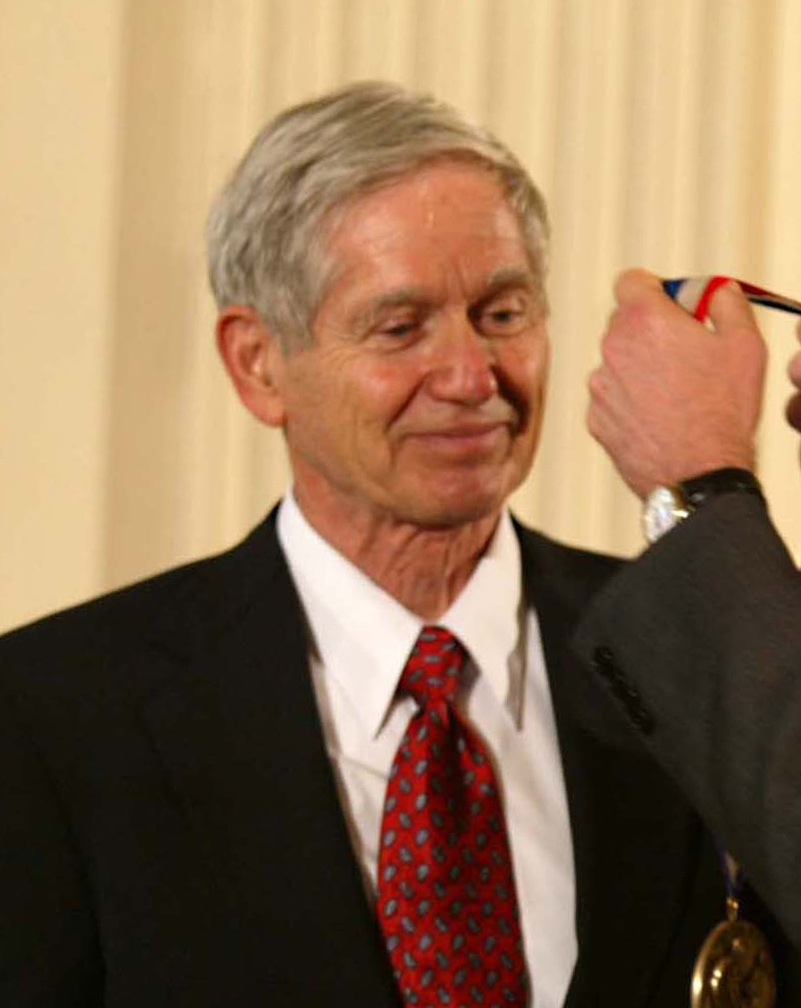
\includegraphics[height=0.5\textheight]{ch0_keeling_2001.jpg}\\[1mm]
\imgcap{Charles David Keeling (1928--2005), 2001}
\imgcredit{https://commons.wikimedia.org/wiki/File:Charles_David_Keeling_2001.jpg}{Photo: National Science Foundation (2001); public domain; Wikimedia Commons}
\end{column}
\end{columns}
\end{frame}

\begin{frame}{Atmospheric CO2 at Mauna Loa}
\itemsize{\footnotesize}
\begin{center}
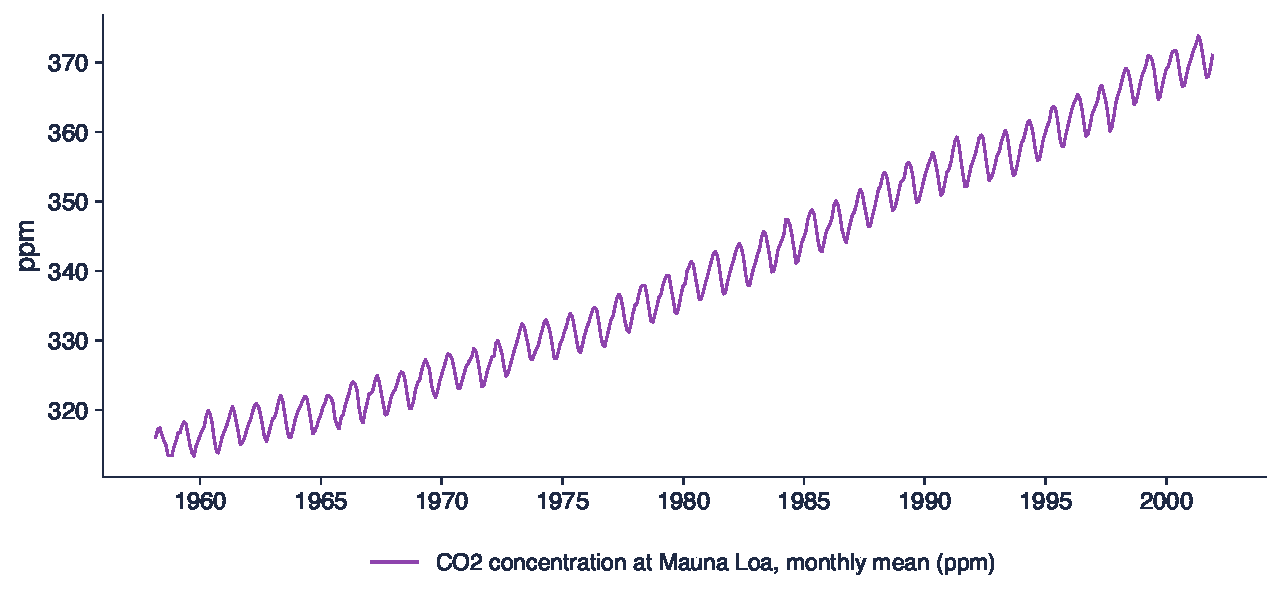
\includegraphics[width=0.94\textwidth,height=0.58\textheight,keepaspectratio]{tsa_ch0_co2.pdf}
\end{center}
\vspace{-2mm}
\begin{itemize}
    \item Monthly averages of the weekly measurements, March 1958 -- December 2001 (526 months; the classic data set of statsmodels)
\end{itemize}
\quantlet{TSA\_ch0\_examples}{\qlurl{TSA_ch0_examples}}
\end{frame}

\begin{frame}{Interpretation: CO2}
\itemsize{\small}
\begin{itemize}
    \item \textbf{Trend}: from 316.1 to 371.0 ppm
    \begin{itemize}
        \item on average 1.26 ppm a year; the slope itself increases over time
    \end{itemize}
    \item \textbf{Seasonality}: a regular yearly wave of a few ppm
    \begin{itemize}
        \item the wave keeps roughly its size while the level rises: an additive pattern
    \end{itemize}
    \item \textbf{Almost no noise}
    \begin{itemize}
        \item a careful physical measurement, unlike GDP or exchange rates
    \end{itemize}
    \item A smooth series with a clear trend and season: the easiest case for decomposition and smoothing
\end{itemize}
\end{frame}

\begin{frame}{Patterns in Six Series}
\itemsize{\footnotesize}
\begin{center}
\scriptsize
\begin{tabular}{lllll}
\toprule
\textbf{Series} & \textbf{Trend} & \textbf{Season} & \textbf{Cycle} & \textbf{Noise} \\
\midrule
GDP (unadjusted) & up & strong, multiplicative & recessions & small \\
Inflation rate & down after 1997 & removed by the 12-month rate & shocks & medium \\
EUR/RON & stochastic & -- & -- & medium \\
BET & up, with crashes & -- & booms and busts & large \\
Electricity & down & strong, winter peak & -- & medium \\
CO2 & up, accelerating & regular, additive & -- & very small \\
\bottomrule
\end{tabular}
\end{center}
\begin{itemize}
    \item \textbf{Question for the room}: which of these series would you forecast most accurately one year ahead?
    \pause
    \item \textbf{Answer}: CO2: a smooth trend and a stable season, little noise; the BET is the hardest: no season and large noise
\end{itemize}
\end{frame}

\begin{frame}{Recap: Time series on real data}
\itemsize{\small}
\begin{itemize}
    \item GDP and electricity: trend plus a strong seasonal pattern; GDP also shows recessions
    \item Inflation: the 12-month rate removes the season but reacts late
    \item EUR/RON and the BET: trends built from shocks, no seasonality, hard to forecast
    \item CO2: a smooth trend and an additive yearly wave
    \item Look at the chart first: it decides the model
\end{itemize}
\end{frame}


%=============================================================================
\section{A Short History}
%=============================================================================

\begin{frame}{Sunspots: the First Famous Time Series}
\itemsize{\footnotesize}
\begin{columns}[T]
\begin{column}{0.30\textwidth}
\centering
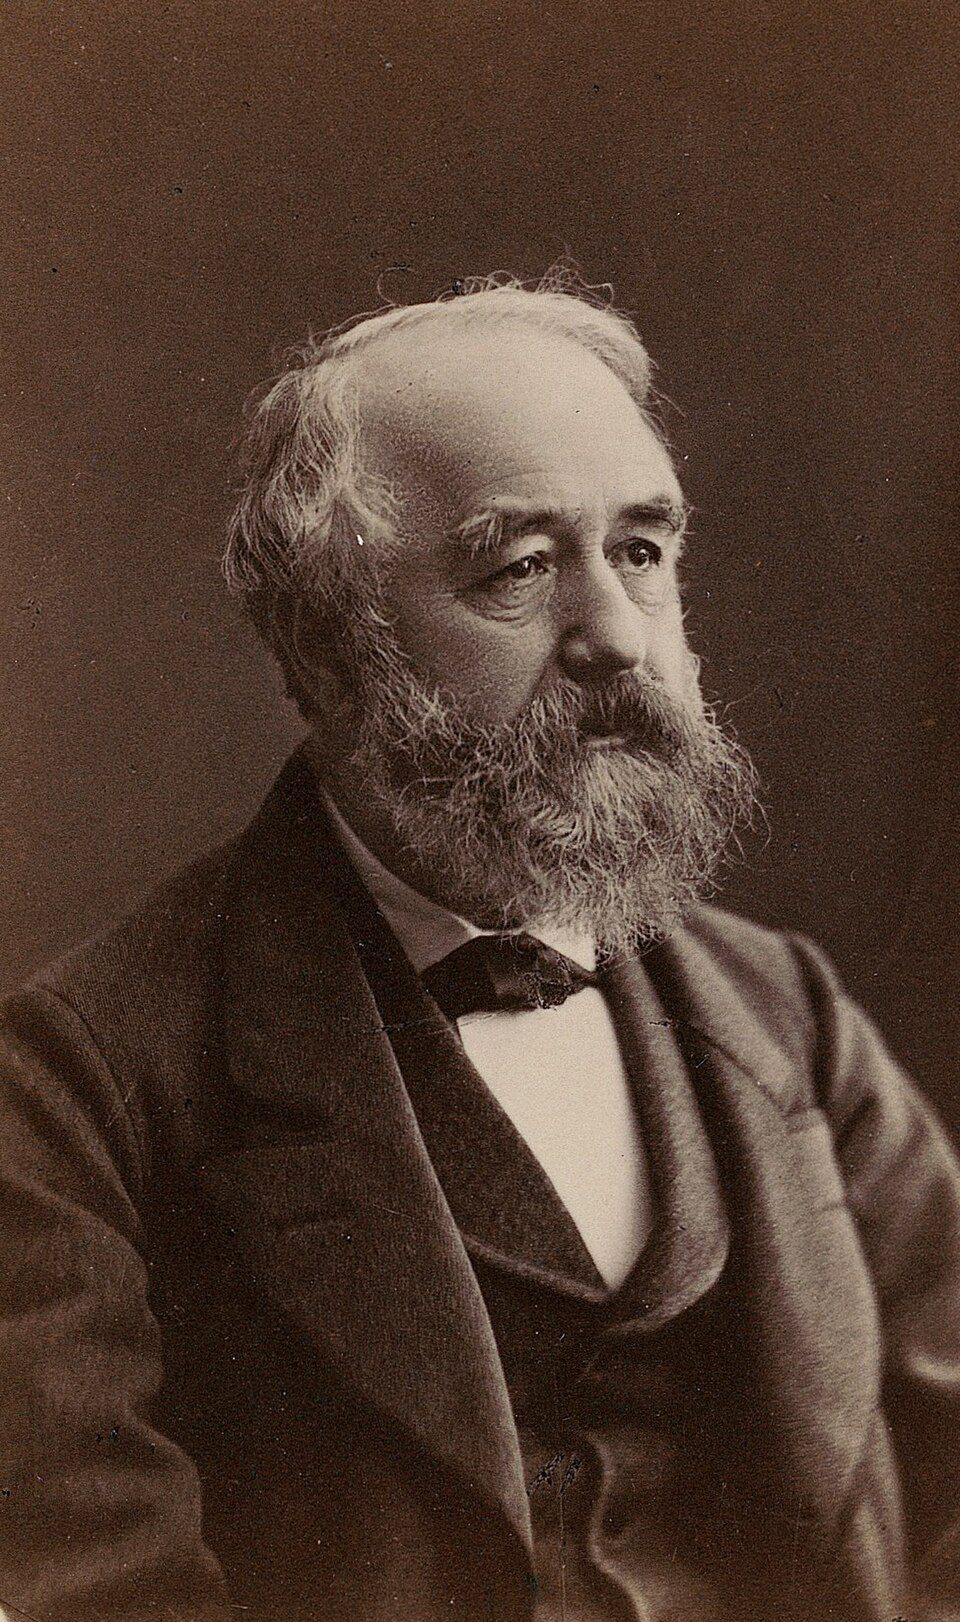
\includegraphics[height=0.42\textheight]{ch0_wolf.jpg}\\[1mm]
\imgcap{Rudolf Wolf (1816--1893)}
\imgcredit{https://commons.wikimedia.org/wiki/File:ETH-BIB-Wolf,_Johann_Rudolf_(1816-1893)-Portrait-Portr_12033-RE.tif_(cropped).jpg}{Photo: Emil Gassler (1888--1893); public domain; ETH-Bibliothek, Wikimedia Commons}
\end{column}
\begin{column}{0.66\textwidth}
\begin{itemize}
    \item \textbf{1848}: the Swiss astronomer Rudolf Wolf defines a daily index of solar activity from the number of sunspots
    \item he reconstructs it back to 1749: the Wolf (later Wolfer) sunspot numbers
    \item the series rises and falls in waves of about 11 years, but neither the length nor the height of the waves is constant
    \item the question: a hidden periodic signal plus noise, or something else?
\end{itemize}
\centering
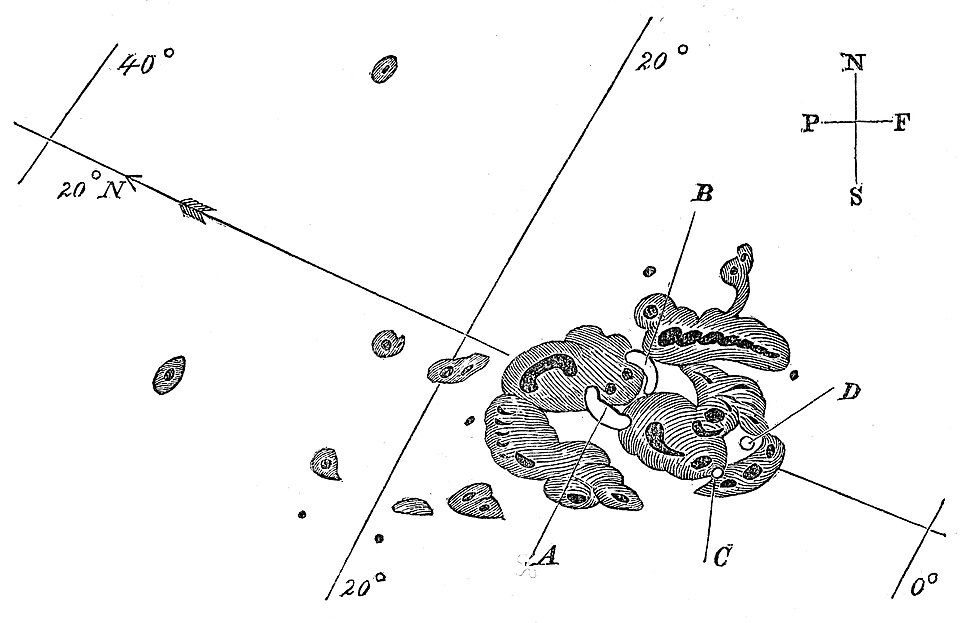
\includegraphics[height=0.26\textheight]{ch0_sunspots_1859.jpg}\\[1mm]
\imgcap{Sunspots drawn by Richard Carrington, 1 September 1859}
\imgcredit{https://commons.wikimedia.org/wiki/File:Carrington_Richard_drawing_of_1859_sunspots.jpeg}{Drawing: Richard Carrington (1859); public domain; Wikimedia Commons}
\end{column}
\end{columns}
\end{frame}

\begin{frame}{Yule (1926, 1927): Dependence Is the Model}
\itemsize{\small}
\begin{itemize}
    \item \textbf{1926}: \emph{nonsense correlations} between time series (\refYuleNonsense)
    \begin{itemize}
        \item two unrelated series with trends can show a correlation close to 1
        \item his example: the share of Church of England marriages and the mortality rate in England and Wales
        \item today: spurious regression (Chapter 3) and cointegration (Chapter 7)
    \end{itemize}
    \item \textbf{1927}: Wolfer's sunspot numbers explained by their own past (\refYule)
    \begin{itemize}
        \item instead of hidden sine waves: $y_t = \phi_1 y_{t-1} + \phi_2 y_{t-2} + \varepsilon_t$, with random disturbances $\varepsilon_t$
        \item the first \textbf{autoregressive} model: AR(2) (Chapter 2)
        \item disturbances shift the waves, so the period drifts, as in the data
    \end{itemize}
\end{itemize}
\end{frame}

\begin{frame}{Slutsky (1937): Cycles from Random Shocks}
\itemsize{\footnotesize}
\begin{columns}[T]
\begin{column}{0.28\textwidth}
\centering
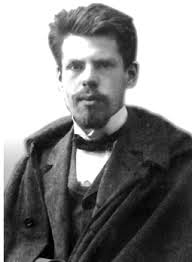
\includegraphics[height=0.42\textheight]{ch0_slutsky.jpg}\\[1mm]
\imgcap{Eugen Slutsky (1880--1948)}
\imgcredit{https://commons.wikimedia.org/wiki/File:\%D0\%A1\%D0\%BB\%D1\%83\%D1\%86\%D1\%8C\%D0\%BA\%D0\%B8\%D0\%B9_\%D0\%84\%D0\%B2\%D0\%B3\%D0\%B5\%D0\%BD.jpg}{Photo: unknown author; public domain; Wikimedia Commons}
\end{column}
\begin{column}{0.68\textwidth}
\begin{itemize}
    \item \textbf{1927} (Moscow), \textbf{1937} in English: \emph{The summation of random causes as the source of cyclic processes} (\refSlutsky)
    \item \textbf{The experiment}
    \begin{itemize}
        \item take independent random numbers (the digits of a lottery draw)
        \item replace each one by the sum of the last 10: $y_t = \varepsilon_t + \varepsilon_{t-1} + \cdots + \varepsilon_{t-9}$
        \item the result looks like business cycles
    \end{itemize}
    \item Today this is a \textbf{moving-average} process: MA(9) (Chapter 2)
\end{itemize}
\end{column}
\end{columns}
\end{frame}

\begin{frame}{Slutsky's Experiment, Simulated}
\itemsize{\footnotesize}
\begin{center}
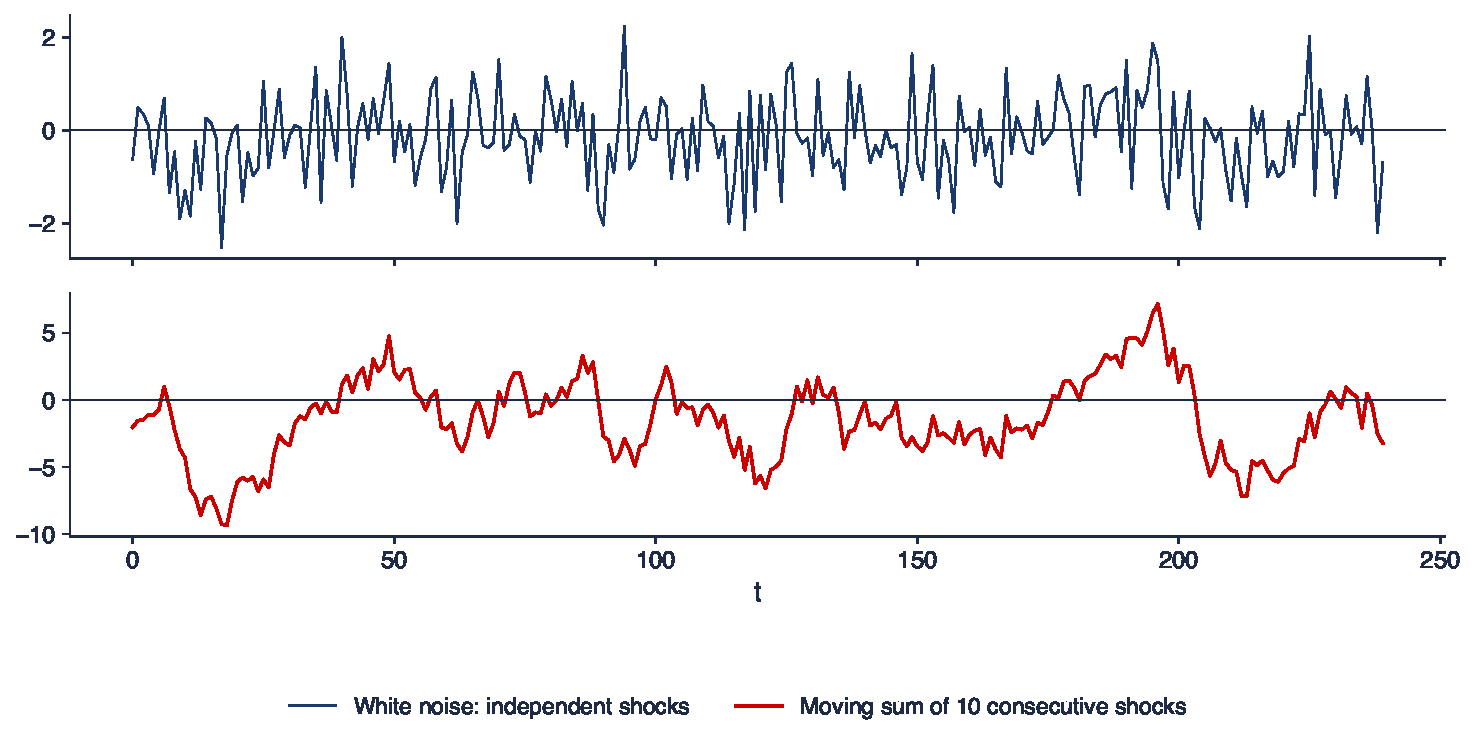
\includegraphics[width=0.94\textwidth,height=0.58\textheight,keepaspectratio]{tsa_ch0_slutsky.pdf}
\end{center}
\vspace{-2mm}
\begin{itemize}
    \item Top: 240 independent shocks with the standard Normal distribution; bottom: the moving sum of 10 consecutive shocks
\end{itemize}
\quantlet{TSA\_ch0\_slutsky}{\qlurl{TSA_ch0_slutsky}}
\end{frame}

\begin{frame}{Interpretation: Slutsky's Experiment}
\itemsize{\small}
\begin{itemize}
    \item \textbf{No cycle was put in, yet waves appear}
    \begin{itemize}
        \item the moving sum crosses zero upwards 16 times in 240 periods: waves of irregular length
        \item neighbouring values share 9 of their 10 shocks, so they are strongly correlated
    \end{itemize}
    \item \textbf{Two lessons}
    \begin{itemize}
        \item a cycle in a chart is not proof of a periodic cause
        \item smoothing (moving averages) can \emph{create} apparent cycles: be careful with smoothed data
    \end{itemize}
    \item Yule (AR) and Slutsky (MA) gave the two building blocks of the ARMA models
\end{itemize}
\end{frame}

\begin{frame}{Kolmogorov and Wiener: the Best Linear Forecast}
\itemsize{\footnotesize}
\begin{columns}[T]
\begin{column}{0.48\textwidth}
\centering
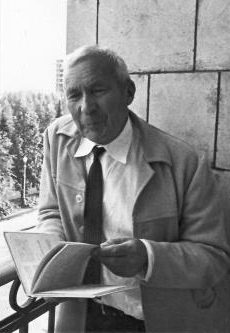
\includegraphics[height=0.36\textheight]{ch0_kolmogorov.jpg}\\[1mm]
\imgcap{Andrei Kolmogorov (1903--1987)}
\imgcredit{https://commons.wikimedia.org/wiki/File:Andrej_Nikolajewitsch_Kolmogorov.jpg}{Photo: Konrad Jacobs; CC BY-SA 2.0 de; Oberwolfach, Wikimedia Commons}\\[1mm]
\raggedright
\begin{itemize}
    \item \textbf{1941}: the theory of interpolation and extrapolation of stationary sequences (\refKolmogorov)
\end{itemize}
\end{column}
\begin{column}{0.48\textwidth}
\centering
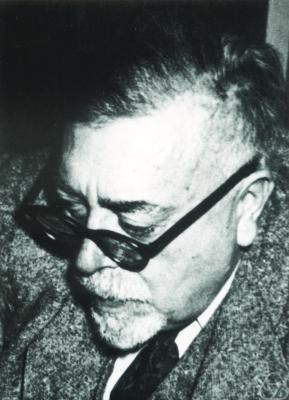
\includegraphics[height=0.36\textheight]{ch0_wiener.jpg}\\[1mm]
\imgcap{Norbert Wiener (1894--1964)}
\imgcredit{https://commons.wikimedia.org/wiki/File:Norbert_wiener.jpg}{Photo: Konrad Jacobs; CC BY-SA 2.0 de; Oberwolfach, Wikimedia Commons}\\[1mm]
\raggedright
\begin{itemize}
    \item \textbf{1942} (classified report), \textbf{1949}: the Wiener filter, developed for anti-aircraft fire control (\refWiener)
\end{itemize}
\end{column}
\end{columns}
\begin{itemize}
    \item Both answer: which weighted sum of past values forecasts the future with the smallest mean squared error? The ancestor of the Kalman filter (Chapter 10)
\end{itemize}
\end{frame}

\begin{frame}{Box and Jenkins (1970): a Method for Practice}
\itemsize{\footnotesize}
\begin{columns}[T]
\begin{column}{0.62\textwidth}
\begin{itemize}
    \item \textbf{1970}: George Box and Gwilym Jenkins publish \emph{Time Series Analysis: Forecasting and Control} (\refBJ)
    \item \textbf{The Box--Jenkins cycle}
    \begin{itemize}
        \item \textbf{identify}: choose a model from charts and the ACF
        \item \textbf{estimate}: fit its parameters
        \item \textbf{check}: are the residuals unpredictable noise?
        \item \textbf{forecast}: only when the checks pass
    \end{itemize}
    \item ARIMA models and their seasonal version SARIMA come from this book (Chapters 2--4)
    \item Box: \emph{all models are wrong, but some are useful}
\end{itemize}
\end{column}
\begin{column}{0.34\textwidth}
\centering
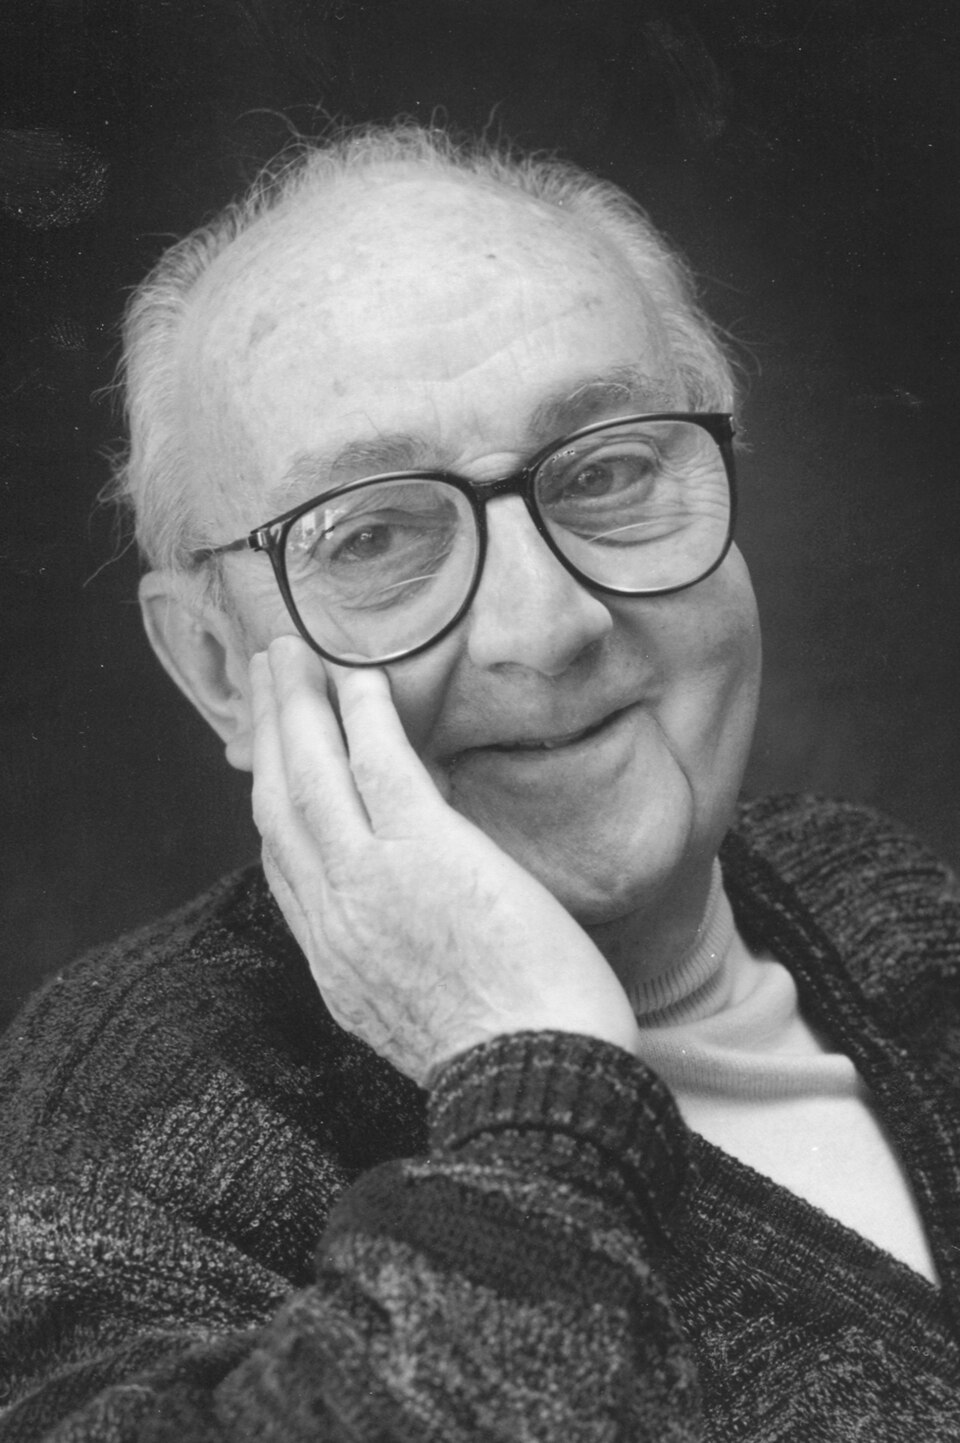
\includegraphics[height=0.52\textheight]{ch0_box.jpg}\\[1mm]
\imgcap{George E.P.\ Box (1919--2013)}
\imgcredit{https://commons.wikimedia.org/wiki/File:GeorgeEPBox_(cropped).jpg}{Photo: DavidMCEddy (2011); CC BY-SA 3.0; Wikimedia Commons}
\end{column}
\end{columns}
\end{frame}

\begin{frame}{A Century in One Line}
\itemsize{\scriptsize}
\centering
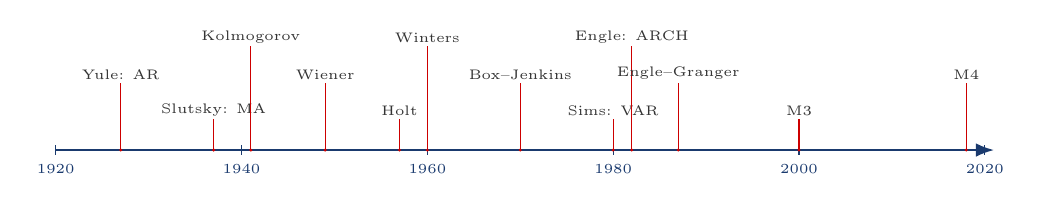
\begin{tikzpicture}[x=0.118cm, y=0.62cm, font=\tiny]
\draw[thick, MainBlue, -{Latex}] (0,0) -- (101,0);
\foreach \x/\y in {0/1920, 20/1940, 40/1960, 60/1980, 80/2000, 100/2020} { \draw[MainBlue] (\x,0.1) -- (\x,-0.1); \node[below, text=MainBlue] at (\x,-0.1) {\y}; }
\foreach \x/\l/\h in {7/{Yule: AR}/1.5, 17/{Slutsky: MA}/0.75, 21/{Kolmogorov}/2.25, 29/{Wiener}/1.5, 37/{Holt}/0.75, 40/{Winters}/2.25, 50/{Box--Jenkins}/1.5, 60/{Sims: VAR}/0.75, 62/{Engle: ARCH}/2.25, 67/{Engle--Granger}/1.5, 80/{M3}/0.75, 98/{M4}/1.5} {
  \draw[IDAred] (\x,0) -- (\x,\h-0.12); \fill[IDAred] (\x,0) circle (0.6pt);
  \node[above, text=DarkGray, inner sep=1pt] at (\x,\h-0.12) {\l};
}
\end{tikzpicture}
\begin{itemize}
    \item 1927 Yule, 1937 Slutsky, 1941 Kolmogorov, 1949 Wiener: the foundations (\tsachlink{https://danpele.github.io/Time-Series-Analysis/EN/Courses/chapter1_stochastic_processes_stationarity.pdf}{Chapters 1} and 2)
    \item 1957 \refHolt, 1960 \refWinters: exponential smoothing, born in industry for sales and inventories (this chapter)
    \item 1970 Box--Jenkins (Chapters 2--4); 1980 \refSims\ (Chapter 6); 1982 \refEngle\ (Chapter 5); 1987 \refEG\ (Chapter 7)
    \item 2000 and 2020: the M3 and M4 forecasting competitions compare methods on thousands of real series (\refMthree; \refMfour)
\end{itemize}
\end{frame}

\begin{frame}{Recap: a short history}
\itemsize{\small}
\begin{itemize}
    \item Sunspots (Wolf, 1848) posed the first question: hidden periods or random dependence?
    \item Yule: a series explained by its own past (AR); Slutsky: sums of shocks look like cycles (MA)
    \item Kolmogorov and Wiener: the optimal linear forecast
    \item Box and Jenkins: identify, estimate, check, forecast
    \item Forecasting competitions: simple methods are hard to beat
\end{itemize}
\end{frame}


%=============================================================================
\section{Components and Decomposition}
%=============================================================================

\begin{frame}{Four Components}
\itemsize{\small}
\begin{itemize}
    \item \textbf{Trend} $T_t$: the long-run movement of the level
    \begin{itemize}
        \item GDP growth, the rise of CO2; it can change direction slowly
    \end{itemize}
    \item \textbf{Seasonality} $S_t$: a pattern that repeats with a \textbf{fixed, known period} $m$
    \begin{itemize}
        \item $m = 4$ for quarterly data, $m = 12$ for monthly data, $m = 7$ for daily data with a weekly pattern
    \end{itemize}
    \item \textbf{Cycle} $C_t$: rises and falls \textbf{without a fixed period}, usually longer than a year
    \begin{itemize}
        \item business cycles: expansions and recessions of 2--10 years; usually merged with the trend into a \textbf{trend-cycle}
    \end{itemize}
    \item \textbf{Remainder} $R_t$ (irregular component, noise): what is left
    \begin{itemize}
        \item it should look unpredictable; if it does not, the decomposition missed something
    \end{itemize}
\end{itemize}
\end{frame}

\begin{frame}{Cycle or Seasonality?}
\itemsize{\small}
\begin{itemize}
    \item \textbf{Question for the room}: electricity generation is high every January
    \begin{itemize}
        \item is this a cycle or seasonality?
    \end{itemize}
    \pause
    \item \textbf{Answer}: seasonality: the period is fixed (12 months) and known in advance
    \begin{itemize}
        \item a recession arrives at an unknown moment and lasts an unknown time: that is a cycle
    \end{itemize}
    \item \textbf{Why the difference matters}
    \begin{itemize}
        \item seasonality can be forecast years ahead: next January will again be high
        \item cycles are hard to forecast: their timing changes (Slutsky)
        \item sunspots: an 11-year \emph{cycle}, not a season, because its length varies
    \end{itemize}
\end{itemize}
\end{frame}

\begin{frame}{Additive and Multiplicative Models}
\itemsize{\small}
\begin{itemize}
    \item \textbf{Additive}: $y_t = T_t + S_t + R_t$
    \begin{itemize}
        \item the seasonal swing has a constant size in units of $y$ (CO2: a few ppm every year)
    \end{itemize}
    \item \textbf{Multiplicative}: $y_t = T_t \times S_t \times R_t$
    \begin{itemize}
        \item the seasonal swing is a constant \textbf{percentage} of the level (GDP: Q1 about a quarter below the trend)
        \item $S_t$ and $R_t$ are factors around 1: $S_t = 0.8$ means 20\% below the trend
    \end{itemize}
    \item \textbf{The logarithm links them}: $\ln y_t = \ln T_t + \ln S_t + \ln R_t$
    \begin{itemize}
        \item a multiplicative series becomes additive after taking logs
    \end{itemize}
    \item \textbf{How to choose}: look at the chart
    \begin{itemize}
        \item does the seasonal swing grow with the level? Multiplicative (or logs); otherwise additive
    \end{itemize}
\end{itemize}
\end{frame}

\begin{frame}{Centred Moving Averages}
\itemsize{\small}
\begin{itemize}
    \item \textbf{Moving average of order} $k$ (odd): the mean of $k$ neighbouring values
    \begin{itemize}
        \item $\hat T_t = \frac{1}{k} \sum_{j=-q}^{q} y_{t+j}$, with $k = 2q + 1$; it smooths out the noise
    \end{itemize}
    \item \textbf{The key property}: a moving average over one full season removes the seasonal pattern
    \begin{itemize}
        \item every quarter enters once, so the seasonal effects cancel out
    \end{itemize}
    \item \textbf{Even period} $m = 4$: a $2 \times 4$ moving average, to stay centred on a quarter
    \begin{itemize}
        \item $\hat T_t = \frac{1}{8} y_{t-2} + \frac{1}{4} y_{t-1} + \frac{1}{4} y_t + \frac{1}{4} y_{t+1} + \frac{1}{8} y_{t+2}$
        \item five quarters, the two ends with half weight; for monthly data, $2 \times 12$
    \end{itemize}
    \item The first and the last $m/2$ values have no centred average: the trend estimate is missing at both ends
\end{itemize}
\end{frame}

\begin{frame}{Worked Example: a $2 \times 4$ Moving Average}
\itemsize{\footnotesize}
\begin{columns}[T]
\begin{column}{0.32\textwidth}
\begin{center}
\footnotesize
\begin{tabular}{lr}
\toprule
\textbf{Quarter} & \textbf{$y_t$} \\
\midrule
2024 Q1 & 38.7 \\
2024 Q2 & 45.6 \\
2024 Q3 & 52.8 \\
2024 Q4 & 59.2 \\
2025 Q1 & 38.9 \\
\bottomrule
\end{tabular}
\end{center}

\end{column}
\begin{column}{0.64\textwidth}
\begin{itemize}
    \item Romanian real GDP, billion EUR (Eurostat, unadjusted)
    \item \textbf{Trend in 2024 Q3}
    \begin{itemize}
        \item $\hat T = \frac{1}{4}\left(\frac{38.7}{2} + 45.6 + 52.8 + 59.2 + \frac{38.9}{2}\right) = $ 49.10
    \end{itemize}
    \item \textbf{Seasonal ratio}
    \begin{itemize}
        \item $y / \hat T = 52.8 / $ 49.10: the third quarter is above the trend
    \end{itemize}
    \item Averaging such ratios over all years gives the seasonal factor of each quarter
\end{itemize}
\end{column}
\end{columns}
\end{frame}

\begin{frame}{Classical Decomposition, Step by Step}
\itemsize{\small}
\begin{itemize}
    \item \textbf{Step 1}: trend-cycle $\hat T_t$ by a centred $2 \times m$ moving average
    \item \textbf{Step 2}: detrend
    \begin{itemize}
        \item multiplicative: $y_t / \hat T_t$; additive: $y_t - \hat T_t$
    \end{itemize}
    \item \textbf{Step 3}: seasonal factors $\hat S_1, \ldots, \hat S_m$
    \begin{itemize}
        \item average the detrended values of each season over all years
        \item normalise: they average to 1 (multiplicative) or to 0 (additive)
    \end{itemize}
    \item \textbf{Step 4}: remainder $\hat R_t = y_t / (\hat T_t \hat S_t)$ or $y_t - \hat T_t - \hat S_t$
    \item \textbf{Seasonally adjusted series}: $y_t / \hat S_t$ or $y_t - \hat S_t$
    \begin{itemize}
        \item limits: the same season every year, no trend at the ends, sensitive to outliers
    \end{itemize}
\end{itemize}
\end{frame}

\begin{frame}{Decomposition of the Romanian GDP}
\itemsize{\footnotesize}
\begin{center}
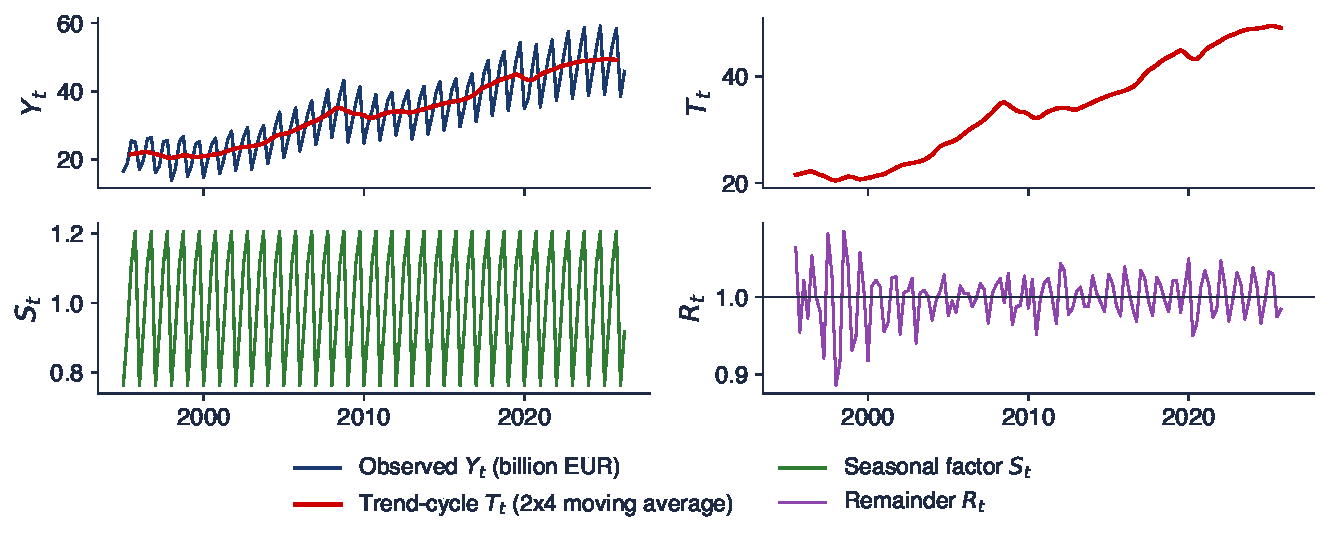
\includegraphics[width=0.94\textwidth,height=0.66\textheight,keepaspectratio]{tsa_ch0_components.pdf}
\end{center}
\vspace{-2mm}
\begin{itemize}
    \item Classical multiplicative decomposition, $m = 4$: observed series and trend-cycle, trend-cycle, seasonal factors, remainder
\end{itemize}
\quantlet{TSA\_ch0\_decomposition}{\qlurl{TSA_ch0_decomposition}}
\end{frame}

\begin{frame}{Interpretation: Seasonal Factors of GDP}
\itemsize{\footnotesize}
\begin{columns}[T]
\begin{column}{0.36\textwidth}
\begin{center}
\footnotesize
\begin{tabular}{lrr}
\toprule
\textbf{Quarter} & $\hat S_q$ & relative to trend \\
\midrule
Q1 & 0.762 & -23.8\% \\
Q2 & 0.918 & -8.2\% \\
Q3 & 1.113 & $+$11.3\% \\
Q4 & 1.207 & $+$20.7\% \\
\bottomrule
\end{tabular}
\end{center}

\end{column}
\begin{column}{0.60\textwidth}
\begin{itemize}
    \item \textbf{Reading the factors}
    \begin{itemize}
        \item a typical first quarter is -23.8\% below the trend, a typical fourth quarter $+$20.7\% above it
        \item Q4 is about 58\% larger than Q1 for purely seasonal reasons
    \end{itemize}
    \item \textbf{Remainder}
    \begin{itemize}
        \item standard deviation about 3.3\%; larger in the 1990s and in 2020
    \end{itemize}
    \item Consequence: compare a quarter with the same quarter of the previous year, never with the previous quarter of the raw series
\end{itemize}
\end{column}
\end{columns}
\end{frame}

\begin{frame}{STL: a Flexible Decomposition}
\itemsize{\small}
\begin{itemize}
    \item \textbf{STL}: Seasonal and Trend decomposition using LOESS (\refSTL)
    \begin{itemize}
        \item LOESS (locally estimated scatterplot smoothing): a weighted regression fitted around each point
    \end{itemize}
    \item \textbf{Advantages over the classical method}
    \begin{itemize}
        \item the seasonal pattern may change slowly from year to year
        \item a trend estimate up to the last observation
        \item a robust version: outliers go into the remainder and do not distort the season
    \end{itemize}
    \item \textbf{Limits}
    \begin{itemize}
        \item additive only: use it on $\ln y_t$ for multiplicative series
        \item no calendar effects (working days, Easter)
    \end{itemize}
    \item Statistical offices use X-13ARIMA-SEATS or TRAMO-SEATS, which build on ARIMA models (Chapter 4)
\end{itemize}
\end{frame}

\begin{frame}{STL Decomposition of CO2}
\itemsize{\footnotesize}
\begin{center}
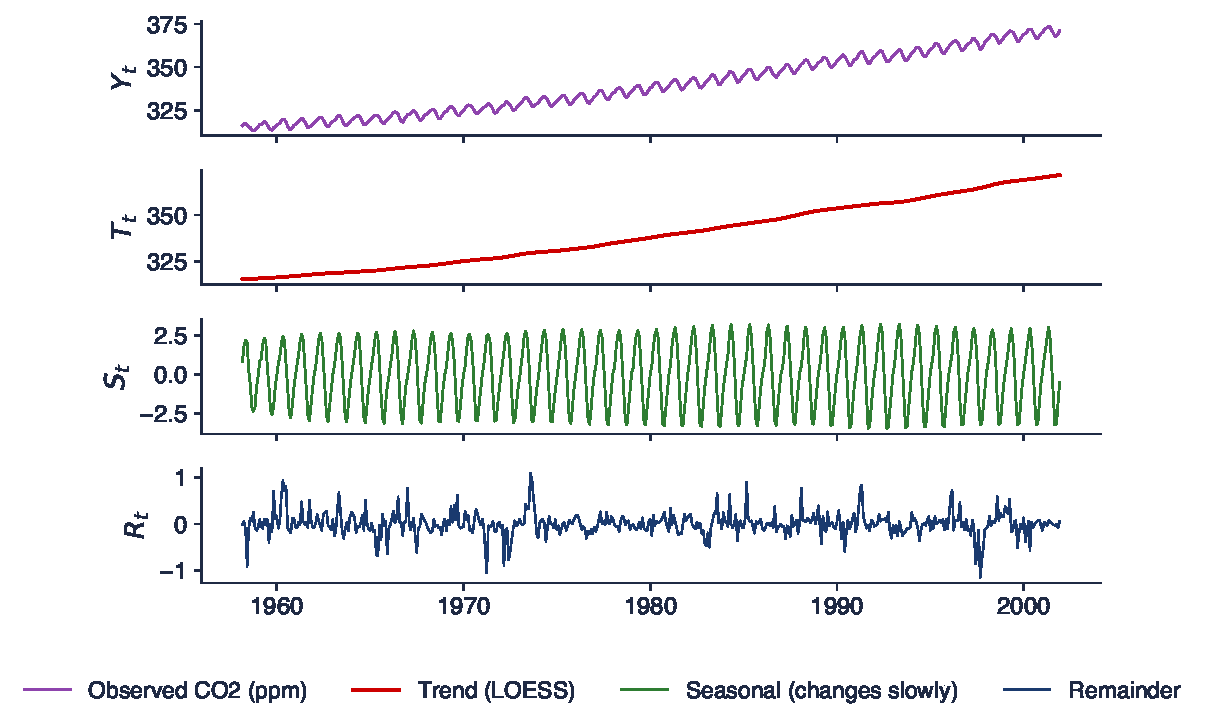
\includegraphics[width=0.94\textwidth,height=0.66\textheight,keepaspectratio]{tsa_ch0_stl.pdf}
\end{center}
\vspace{-2mm}
\begin{itemize}
    \item Robust STL with period 12 on the monthly CO2 series: observed, trend, seasonal, remainder (ppm)
\end{itemize}
\quantlet{TSA\_ch0\_decomposition}{\qlurl{TSA_ch0_decomposition}}
\end{frame}

\begin{frame}{Interpretation: STL of CO2}
\itemsize{\small}
\begin{itemize}
    \item \textbf{Trend}: smooth, slightly convex: the rise accelerates
    \item \textbf{Seasonal}: maximum in May, minimum in October
    \begin{itemize}
        \item winter and spring: decay of fallen leaves releases CO2; summer: photosynthesis absorbs it
        \item the yearly range grows from 4.9 ppm (1959) to 6.3 ppm (2001): STL lets the season change
    \end{itemize}
    \item \textbf{Remainder}: standard deviation 0.25 ppm
    \begin{itemize}
        \item small compared with the season: trend and season explain almost everything
        \item check the larger spikes against the history of the station before calling them noise
    \end{itemize}
\end{itemize}
\end{frame}

\begin{frame}{Recap: components and decomposition}
\itemsize{\small}
\begin{itemize}
    \item Trend, seasonality (fixed period), cycle (no fixed period), remainder
    \item Additive if the seasonal swing is constant, multiplicative if it grows with the level; logs turn one into the other
    \item A centred $2 \times m$ moving average removes the season and estimates the trend-cycle
    \item Romanian GDP: Q1 about -23.8\% and Q4 about $+$20.7\% relative to the trend
    \item STL lets the seasonal pattern change and is robust to outliers
\end{itemize}
\end{frame}


%=============================================================================
\section{Notation, Transformations and the ACF}
%=============================================================================

\begin{frame}{Notation Used in the Course}
\itemsize{\footnotesize}
\begin{center}
\footnotesize
\begin{tabular}{>{\raggedright\arraybackslash}p{3.2cm}>{\raggedright\arraybackslash}p{8.8cm}}
\toprule
\textbf{Symbol} & \textbf{Meaning} \\
\midrule
$y_t$, $t = 1, \ldots, T$ & the observation at time $t$; $T$ observations in the sample \\
$\bar y = \frac1T \sum_t y_t$ & the sample mean \\
$L y_t = y_{t-1}$ & the \textbf{lag operator}: shifts the series back one period; $L^k y_t = y_{t-k}$ \\
$\Delta y_t = y_t - y_{t-1}$ & the \textbf{first difference}, $\Delta = 1 - L$ \\
$\Delta_m y_t = y_t - y_{t-m}$ & the \textbf{seasonal difference}, $\Delta_m = 1 - L^m$ \\
$\hat y_{T+h|T}$ & the forecast of $y_{T+h}$ made with the data up to $T$; $h$ is the \textbf{horizon} \\
$e_t = y_t - \hat y_t$ & the forecast error \\
\bottomrule
\end{tabular}
\end{center}
\begin{itemize}
    \item Hats ($\hat{\ }$) mark estimates and forecasts; Greek letters ($\phi, \theta, \alpha$) mark parameters
\end{itemize}
\end{frame}

\begin{frame}{Transformations: Logs, Differences, Growth Rates}
\itemsize{\footnotesize}
\begin{itemize}
    \item \textbf{Logarithm} $\ln y_t$: stabilises a variance that grows with the level
    \item \textbf{Growth rate over one period}: $g_t = 100\,(y_t / y_{t-1} - 1)$
    \begin{itemize}
        \item log approximation: $100\,\Delta \ln y_t \approx g_t$ for small changes
    \end{itemize}
    \item \textbf{Annual growth rate} of a quarterly series: $100\,(y_t / y_{t-4} - 1)$
    \begin{itemize}
        \item it compares the same quarters, so the season cancels out
    \end{itemize}
    \item \textbf{Worked example}: Romanian GDP, 2024 Q1 = 38.7, 2024 Q4 = 59.2, 2025 Q1 = 38.9
    \begin{itemize}
        \item over one quarter: $100\,(38.9 / 59.2 - 1) \approx -34\%$: not a collapse, only winter
        \item over one year: $100\,(38.9 / 38.7 - 1) \approx +0.5\%$: the economy barely grew
    \end{itemize}
    \item \textbf{Log return} of a price: $r_t = 100\,(\ln P_t - \ln P_{t-1})$, in \%
\end{itemize}
\end{frame}

\begin{frame}{From Prices to Returns: the BET}
\itemsize{\footnotesize}
\begin{center}
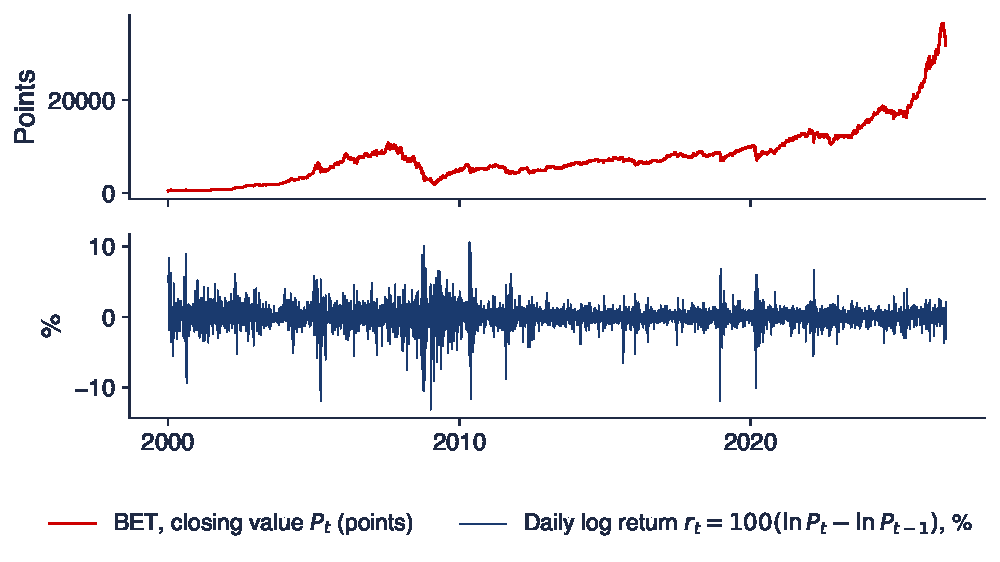
\includegraphics[width=0.94\textwidth,height=0.6\textheight,keepaspectratio]{tsa_ch0_returns.pdf}
\end{center}
\vspace{-2mm}
\begin{itemize}
    \item Top: closing value of the BET since 2000; bottom: daily log returns in \% (6\,670 trading days)
\end{itemize}
\quantlet{TSA\_ch0\_acf}{\qlurl{TSA_ch0_acf}}
\end{frame}

\begin{frame}{Interpretation: Prices and Returns}
\itemsize{\small}
\begin{itemize}
    \item \textbf{The price has a trend; the returns do not}
    \begin{itemize}
        \item returns fluctuate around a mean of 0.064\% a day, with a standard deviation of 1.40\% (about 22\% a year)
    \end{itemize}
    \item \textbf{Extreme days}
    \begin{itemize}
        \item worst: -13.1\% on 7 January 2009; best: +10.6\% on 10 May 2010
    \end{itemize}
    \item \textbf{Calm and turbulent periods alternate}
    \begin{itemize}
        \item large moves cluster in 2008--2010 and in March 2020: \emph{volatility clustering} (Chapter 5)
    \end{itemize}
    \item Differencing the log price removes the trend: most models of the course work on such transformed series
\end{itemize}
\end{frame}

\begin{frame}{The Sample Autocorrelation Function}
\itemsize{\small}
\begin{itemize}
    \item \textbf{Question}: how strongly is $y_t$ related to its own value $k$ periods earlier?
    \item \textbf{Sample autocovariance} at lag $k$
    \begin{itemize}
        \item $c_k = \frac{1}{T} \sum_{t=k+1}^{T} (y_t - \bar y)(y_{t-k} - \bar y)$
    \end{itemize}
    \item \textbf{Sample autocorrelation}: $r_k = c_k / c_0$, between $-1$ and $1$
    \begin{itemize}
        \item the \textbf{ACF} (autocorrelation function) is the sequence $r_1, r_2, \ldots$ plotted against $k$ (the \textbf{correlogram})
    \end{itemize}
    \item \textbf{Reference band} $\pm 1.96 / \sqrt{T}$
    \begin{itemize}
        \item if the series were independent noise, about 95\% of the $r_k$ would fall inside it
        \item the theory (stationarity, white noise, the Ljung--Box test) comes in \tsachlink{https://danpele.github.io/Time-Series-Analysis/EN/Courses/chapter1_stochastic_processes_stationarity.pdf}{Chapter 1}
    \end{itemize}
\end{itemize}
\end{frame}

\begin{frame}{Worked Example: $r_1$ by Hand}
\itemsize{\footnotesize}
\begin{columns}[T]
\begin{column}{0.48\textwidth}
\begin{center}
\footnotesize
\begin{tabular}{rrrr}
\toprule
$t$ & $y_t$ & $y_t - \bar y$ & $(y_t - \bar y)(y_{t-1} - \bar y)$ \\
\midrule
1 & 2 & $-2$ & -- \\
2 & 4 & $0$ & $0$ \\
3 & 3 & $-1$ & $0$ \\
4 & 5 & $1$ & $-1$ \\
5 & 4 & $0$ & $0$ \\
6 & 6 & $2$ & $0$ \\
\midrule sum & 24 & 0 & $-1$ \\
\bottomrule
\end{tabular}
\end{center}

\end{column}
\begin{column}{0.48\textwidth}
\begin{itemize}
    \item $T = 6$, $\bar y = 24 / 6 = 4$
    \item sum of squared deviations: $4 + 0 + 1 + 1 + 0 + 4 = 10$
    \item $r_1 = \dfrac{-1/6}{10/6} = -0.1$
    \item at lag 2: products $(-1)(-2) + (1)(0) + (0)(-1) + (2)(1) = 4$, so $r_2 = 0.4$
    \item \textbf{Interpretation}
    \begin{itemize}
        \item band $\pm 1.96/\sqrt 6 = \pm 0.80$: with 6 observations, neither value is distinguishable from 0
    \end{itemize}
\end{itemize}
\end{column}
\end{columns}
\end{frame}

\begin{frame}{Three Correlograms}
\itemsize{\footnotesize}
\begin{center}
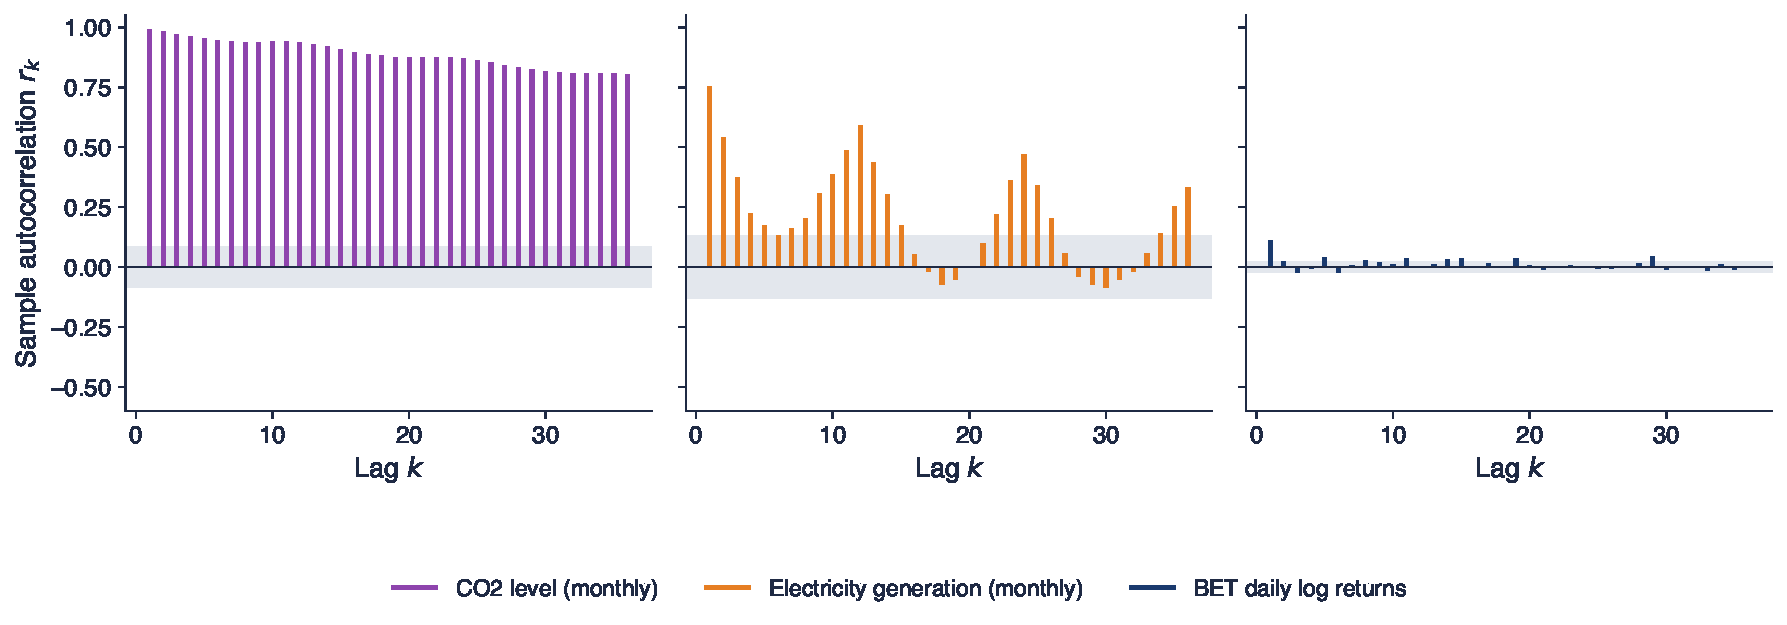
\includegraphics[width=0.94\textwidth,height=0.5\textheight,keepaspectratio]{tsa_ch0_acf.pdf}
\end{center}
\vspace{-2mm}
\begin{itemize}
    \item Sample ACF for lags 1--36; shaded: the band $\pm 1.96/\sqrt{T}$. Left: CO2 level; centre: monthly electricity generation; right: BET daily log returns
\end{itemize}
\quantlet{TSA\_ch0\_acf}{\qlurl{TSA_ch0_acf}}
\end{frame}

\begin{frame}{Interpretation: Three Correlograms}
\itemsize{\small}
\begin{itemize}
    \item \textbf{Trend}: CO2, $r_1 = $ 0.993, still 0.80 at lag 36
    \begin{itemize}
        \item a slow, almost linear decay is the signature of a trend: the level remembers its past for years
    \end{itemize}
    \item \textbf{Seasonality}: electricity, $r_6 = $ 0.13, $r_{12} = $ 0.59
    \begin{itemize}
        \item peaks at 12, 24 and 36 months: this January resembles last January
    \end{itemize}
    \item \textbf{Almost no memory}: BET returns, $r_1 = $ 0.109, $r_2 = $ 0.022, band $\pm$0.024
    \begin{itemize}
        \item small but significant autocorrelations: hard to exploit after trading costs
        \item the \emph{absolute} returns have $r_1 = $ 0.40: the size of moves is predictable, their sign much less (Chapter 5)
    \end{itemize}
    \item The ACF of a level with a trend says little: transform first, then look at the ACF
\end{itemize}
\end{frame}

\begin{frame}{Recap: notation, transformations and the ACF}
\itemsize{\small}
\begin{itemize}
    \item $L y_t = y_{t-1}$, $\Delta = 1 - L$, $\Delta_m = 1 - L^m$; $\hat y_{T+h|T}$ is the forecast for horizon $h$
    \item Logs stabilise the variance; differences remove the trend; annual rates remove the season
    \item $r_k = c_k / c_0$, compared with the band $\pm 1.96/\sqrt T$
    \item Slow decay: trend; peaks at $m, 2m, \ldots$: seasonality; all close to 0: little linear memory
\end{itemize}
\end{frame}


%=============================================================================
\section{Exponential Smoothing}
%=============================================================================

\begin{frame}{Simple Exponential Smoothing (SES)}
\itemsize{\small}
\begin{itemize}
    \item \textbf{Idea}: forecast with a weighted average of the past, recent values weighing more
    \item \textbf{Level equation}: $\ell_t = \alpha y_t + (1 - \alpha)\, \ell_{t-1}$, with $0 < \alpha \le 1$
    \begin{itemize}
        \item forecast for every horizon: $\hat y_{T+h|T} = \ell_T$, a flat line
    \end{itemize}
    \item \textbf{Why ``exponential''}: substituting repeatedly
    \begin{itemize}
        \item $\ell_T = \alpha y_T + \alpha(1-\alpha) y_{T-1} + \alpha(1-\alpha)^2 y_{T-2} + \cdots$
        \item the weights fall geometrically; with $\alpha = 0.5$: 0.5, 0.25, 0.125, \ldots
    \end{itemize}
    \item \textbf{The smoothing constant} $\alpha$
    \begin{itemize}
        \item small $\alpha$: long memory, smooth forecasts, slow reaction; $\alpha = 1$: the naive forecast $\hat y_{T+1} = y_T$
        \item estimated by minimising the sum of squared one-step forecast errors
    \end{itemize}
\end{itemize}
\end{frame}

\begin{frame}{Worked Example: SES with $\alpha = 0.5$}
\itemsize{\footnotesize}
\begin{columns}[T]
\begin{column}{0.52\textwidth}
\begin{center}
\footnotesize
\begin{tabular}{rrrr}
\toprule
$t$ & $y_t$ & $\hat y_{t|t-1} = \ell_{t-1}$ & $\ell_t = 0.5\,y_t + 0.5\,\ell_{t-1}$ \\
\midrule
0 & -- & -- & $\ell_0 = 10$ \\
1 & 10 & 10 & 10 \\
2 & 12 & 10 & 11 \\
3 & 11 & 11 & 11 \\
4 & 13 & 11 & 12 \\
5 & ? & \textbf{12} & -- \\
\bottomrule
\end{tabular}
\end{center}

\end{column}
\begin{column}{0.44\textwidth}
\begin{itemize}
    \item initial level $\ell_0 = 10$ (the first observation)
    \item $t = 2$: $0.5 \times 12 + 0.5 \times 10 = 11$
    \item $t = 4$: $0.5 \times 13 + 0.5 \times 11 = 12$
    \item \textbf{Interpretation}
    \begin{itemize}
        \item the forecast for $t = 5$ and every later period is 12: SES does not extrapolate trends
        \item one-step errors: 0, 2, 0, 2: the forecasts lag behind the rising data
    \end{itemize}
\end{itemize}
\end{column}
\end{columns}
\end{frame}

\begin{frame}{SES on the Monthly EUR/RON}
\itemsize{\footnotesize}
\begin{center}
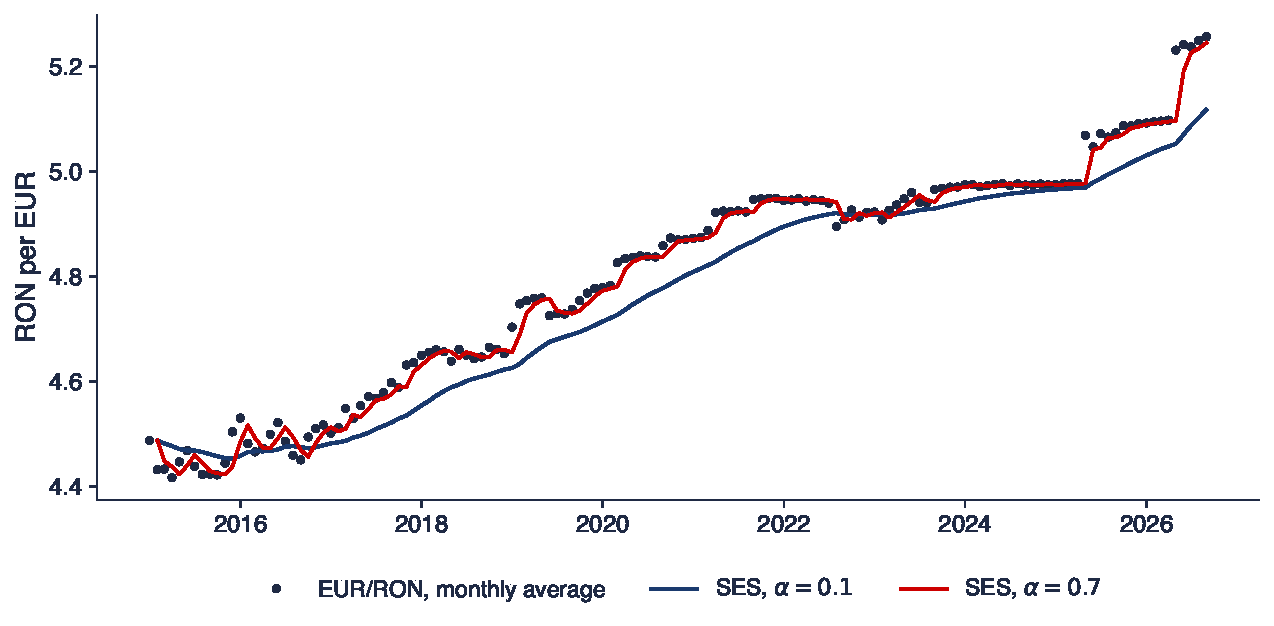
\includegraphics[width=0.94\textwidth,height=0.58\textheight,keepaspectratio]{tsa_ch0_ses.pdf}
\end{center}
\vspace{-2mm}
\begin{itemize}
    \item Dots: monthly averages of the BNR reference rate, January 2015 -- September 2026; lines: one-step SES forecasts $\hat y_{t|t-1}$ with $\alpha = 0.1$ and $\alpha = 0.7$
\end{itemize}
\quantlet{TSA\_ch0\_smoothing}{\qlurl{TSA_ch0_smoothing}}
\end{frame}

\begin{frame}{Interpretation: the Choice of $\alpha$}
\itemsize{\small}
\begin{itemize}
    \item \textbf{$\alpha = 0.1$}: smooth, but always below the rising rate
    \begin{itemize}
        \item it remembers several years: after the jump of 2025 it needs many months to catch up
    \end{itemize}
    \item \textbf{$\alpha = 0.7$}: follows the data closely, one month late
    \item \textbf{Estimated} $\hat\alpha = $ 1.00
    \begin{itemize}
        \item the best SES forecast of next month is this month's average: SES reduces to the naive forecast
        \item typical of exchange rates and prices: the last value contains almost all the information (a random walk, \tsachlink{https://danpele.github.io/Time-Series-Analysis/EN/Courses/chapter1_stochastic_processes_stationarity.pdf}{Chapter 1})
    \end{itemize}
    \item An estimated $\alpha$ near 1 is a finding about the series, not a failure of the method
\end{itemize}
\end{frame}

\begin{frame}{Holt and Holt--Winters}
\itemsize{\footnotesize}
\begin{itemize}
    \item \textbf{Holt (1957)}: level plus a \textbf{trend} $b_t$ (\refHolt)
    \begin{itemize}
        \item $\ell_t = \alpha y_t + (1-\alpha)(\ell_{t-1} + b_{t-1})$, \ $b_t = \beta (\ell_t - \ell_{t-1}) + (1-\beta) b_{t-1}$
        \item forecast: $\hat y_{T+h|T} = \ell_T + h\, b_T$, a straight line; a \textbf{damped} trend flattens it for long horizons
    \end{itemize}
    \item \textbf{Holt--Winters (1960)}: adds seasonal factors $s_t$ with period $m$ (\refWinters)
    \begin{itemize}
        \item multiplicative form: $\hat y_{T+h|T} = (\ell_T + h\, b_T)\, s_{T+h-m}$; each component has its own smoothing constant
    \end{itemize}
    \item \textbf{ETS}: Error, Trend, Seasonal (\refHKSG)
    \begin{itemize}
        \item each method is a statistical model: N (none), A (additive), M (multiplicative), A$_d$ (damped)
        \item e.g.\ ETS(M,A$_d$,M): multiplicative errors, damped trend, multiplicative season; it gives forecast intervals and an information criterion (Chapter 2)
    \end{itemize}
    \item A review of 25 years of exponential smoothing: \refGardner
\end{itemize}
\end{frame}

\begin{frame}{Recap: exponential smoothing}
\itemsize{\small}
\begin{itemize}
    \item SES: $\ell_t = \alpha y_t + (1-\alpha)\ell_{t-1}$; weights decline geometrically; flat forecasts
    \item Small $\alpha$: smooth and slow; $\alpha = 1$: the naive forecast
    \item EUR/RON: $\hat\alpha = $ 1.00, the last value is the best SES forecast
    \item Holt adds a trend, Holt--Winters a season; ETS turns them into statistical models
\end{itemize}
\end{frame}


%=============================================================================
\section{Forecasts and Their Evaluation}
%=============================================================================

\begin{frame}{Forecasting: the Setting}
\itemsize{\small}
\begin{itemize}
    \item \textbf{Forecast} $\hat y_{T+h|T}$: a statement about $y_{T+h}$ made at time $T$
    \begin{itemize}
        \item it may use only the information available at $T$: the \textbf{information set}
        \item $h = 1, 2, \ldots$: the \textbf{horizon}; uncertainty grows with $h$
    \end{itemize}
    \item \textbf{Point and interval forecasts}
    \begin{itemize}
        \item point: one number; interval: a range that contains $y_{T+h}$ with a stated probability (e.g.\ 95\%)
    \end{itemize}
    \item \textbf{What makes a series forecastable}
    \begin{itemize}
        \item a stable pattern (CO2) rather than one driven by news (exchange rates)
        \item a forecast that does not change the outcome: a price forecast published to millions of traders changes the price
    \end{itemize}
\end{itemize}
\end{frame}

\begin{frame}{Four Benchmark Methods}
\itemsize{\small}
\begin{itemize}
    \item \textbf{Mean}: $\hat y_{T+h|T} = \bar y$
    \begin{itemize}
        \item the future looks like the average past
    \end{itemize}
    \item \textbf{Naive}: $\hat y_{T+h|T} = y_T$
    \begin{itemize}
        \item the last value; optimal for a random walk (exchange rates, prices)
    \end{itemize}
    \item \textbf{Seasonal naive}: $\hat y_{T+h|T} = y_{T+h-m}$ (for $h \le m$)
    \begin{itemize}
        \item next January = last January; strong for highly seasonal series
    \end{itemize}
    \item \textbf{Drift}: $\hat y_{T+h|T} = y_T + h\, \dfrac{y_T - y_1}{T - 1}$
    \begin{itemize}
        \item the last value plus the average past change per period
    \end{itemize}
    \item A new model is worth using only if it beats these benchmarks on data it has not seen
\end{itemize}
\end{frame}

\begin{frame}{Training Set and Test Set}
\itemsize{\footnotesize}
\centering
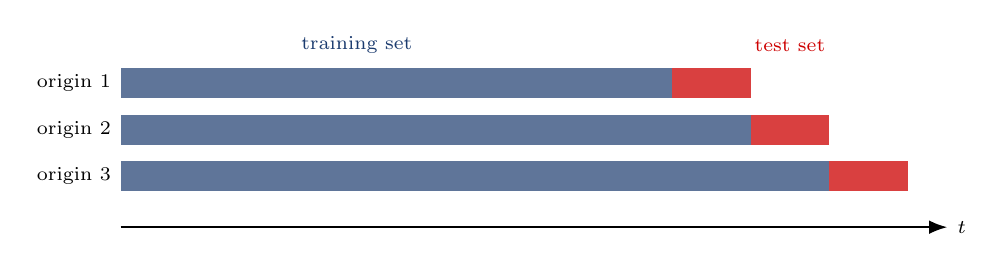
\begin{tikzpicture}[x=0.5cm, y=0.42cm, font=\scriptsize]
\foreach \r/\n in {0/1, 1/2, 2/3} {
  \pgfmathsetmacro{\e}{14 + 2*\r}
  \fill[MainBlue!70] (0, -\r*1.4) rectangle (\e, -\r*1.4 + 0.9);
  \fill[IDAred!75] (\e, -\r*1.4) rectangle (\e + 2, -\r*1.4 + 0.9);
  \node[left] at (0, -\r*1.4 + 0.45) {origin \n};
}
\node[text=MainBlue] at (6, 1.6) {training set};
\node[text=IDAred] at (17, 1.6) {test set};
\draw[-{Latex}, thick] (0, -3.9) -- (21, -3.9) node[right] {$t$};
\end{tikzpicture}
\begin{itemize}
    \item \textbf{Split by time, never at random}
    \begin{itemize}
        \item training set: the first observations, used to choose and fit the method
        \item test set: the last $h$ observations, kept hidden and used only to measure the errors
        \item a random split lets the model see the future: the errors look too small
    \end{itemize}
    \item \textbf{Rolling origin} (time series cross-validation): repeat with the origin moved forward
    \begin{itemize}
        \item average the errors over origins: a more stable estimate of accuracy
    \end{itemize}
\end{itemize}
\end{frame}

\begin{frame}{Measures of Forecast Error}
\itemsize{\footnotesize}
\begin{itemize}
    \item Errors on the test set: $e_{T+j} = y_{T+j} - \hat y_{T+j|T}$, $j = 1, \ldots, h$
    \item \textbf{MAE} (mean absolute error) $= \frac1h \sum_j |e_{T+j}|$
    \begin{itemize}
        \item in the units of the series; easy to explain
    \end{itemize}
    \item \textbf{RMSE} (root mean squared error) $= \sqrt{\frac1h \sum_j e_{T+j}^2}$
    \begin{itemize}
        \item penalises large errors more; always $\ge$ MAE
    \end{itemize}
    \item \textbf{MAPE} (mean absolute percentage error) $= \frac{100}{h} \sum_j |e_{T+j} / y_{T+j}|$
    \begin{itemize}
        \item without units, but useless when $y$ is close to 0 (inflation, returns)
    \end{itemize}
    \item \textbf{MASE} (mean absolute scaled error) $=$ MAE $/$ in-sample MAE of the seasonal naive method (\refHK)
    \begin{itemize}
        \item below 1: better than the seasonal naive method on the training data; comparable across series
    \end{itemize}
\end{itemize}
\end{frame}

\begin{frame}{Worked Example: Errors by Hand}
\itemsize{\footnotesize}
\begin{columns}[T]
\begin{column}{0.46\textwidth}
\begin{center}
\footnotesize
\begin{tabular}{lrrrr}
\toprule
& Q1 & Q2 & Q3 & Q4 \\
\midrule
year 1 & 10 & 14 & 18 & 12 \\
year 2 & 11 & 15 & 20 & 13 \\
\midrule year 3 (test) & 12 & 16 & 21 & 14 \\
naive & 13 & 13 & 13 & 13 \\
seasonal naive & 11 & 15 & 20 & 13 \\
\bottomrule
\end{tabular}
\end{center}

\end{column}
\begin{column}{0.50\textwidth}
\begin{itemize}
    \item \textbf{Naive}: errors $-1, 3, 8, 1$
    \begin{itemize}
        \item MAE $= (1 + 3 + 8 + 1)/4 = 3.25$
        \item RMSE $= \sqrt{(1 + 9 + 64 + 1)/4} = \sqrt{18.75} = 4.33$
    \end{itemize}
    \item \textbf{Seasonal naive}: errors $1, 1, 1, 1$
    \begin{itemize}
        \item MAE $=$ RMSE $= 1$
    \end{itemize}
    \item \textbf{Interpretation}
    \begin{itemize}
        \item the naive forecast misses the season: its large Q3 error dominates the RMSE
        \item on seasonal data, the seasonal naive method is the benchmark to beat
    \end{itemize}
\end{itemize}
\end{column}
\end{columns}
\end{frame}

\begin{frame}{Forecasting Electricity Generation}
\itemsize{\footnotesize}
\begin{center}
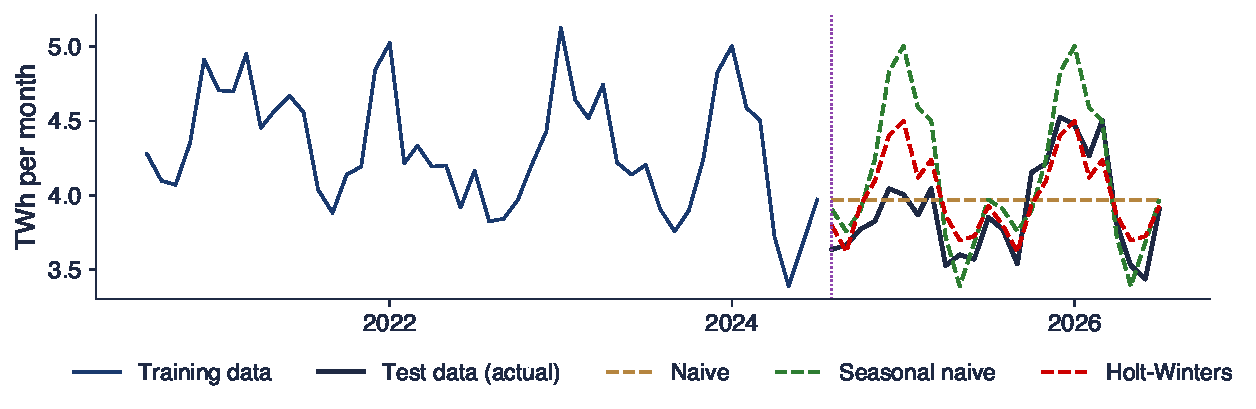
\includegraphics[width=0.94\textwidth,height=0.58\textheight,keepaspectratio]{tsa_ch0_forecast.pdf}
\end{center}
\vspace{-2mm}
\begin{itemize}
    \item Test set: August 2024 -- July 2026 (24 months); training data: all earlier months; dashed: forecasts made once, at the end of the training set
\end{itemize}
\quantlet{TSA\_ch0\_forecast}{\qlurl{TSA_ch0_forecast}}
\end{frame}

\begin{frame}{Interpretation: Which Forecast Wins?}
\itemsize{\footnotesize}
\begin{columns}[T]
\begin{column}{0.50\textwidth}
\begin{center}
\scriptsize
\begin{tabular}{lrrrr}
\toprule
\textbf{Method} & MAE & RMSE & MAPE & MASE \\
\midrule
Naive & 0.28 & 0.33 & 7.3\% & 0.82 \\
Seasonal naive & 0.28 & 0.38 & 7.2\% & 0.83 \\
SES & 0.28 & 0.32 & 7.1\% & 0.81 \\
Holt--Winters & 0.17 & 0.21 & 4.5\% & 0.51 \\
\bottomrule
\end{tabular}
\end{center}
\begin{itemize}
    \item MAE and RMSE in TWh per month
\end{itemize}
\end{column}
\begin{column}{0.46\textwidth}
\begin{itemize}
    \item \textbf{Holt--Winters} has the smallest error on every measure
    \begin{itemize}
        \item it combines a falling level with the winter peak
    \end{itemize}
    \item \textbf{The seasonal naive method is not better than the naive one here}
    \begin{itemize}
        \item it copies the high winter of 2023--2024 into a lower 2024--2026
    \end{itemize}
    \item One test period of 24 months is one sample: a rolling origin gives a firmer answer
\end{itemize}
\end{column}
\end{columns}
\end{frame}

\begin{frame}{Case Study: the M4 Competition}
\itemsize{\footnotesize}
\begin{itemize}
    \item \textbf{The question}: which forecasting methods work best on real data?
    \begin{itemize}
        \item the M competitions, started by Spyros Makridakis in 1982: forecasts submitted blind, scored on hidden test data
    \end{itemize}
    \item \textbf{M4 (2018)}: 100\,000 series (yearly to hourly), 61 methods (\refMfour)
    \begin{itemize}
        \item 12 of the 17 most accurate methods were \textbf{combinations} of several methods
        \item the winner was a hybrid of exponential smoothing and a neural network
        \item pure machine learning methods did poorly: none beat a simple combination of exponential smoothing methods
    \end{itemize}
    \item \textbf{Why it matters for this course}
    \begin{itemize}
        \item benchmarks first; accuracy measured out of sample, on many series rather than one
        \item the same lesson appeared in M3 (\refMthree): complex is not automatically better
    \end{itemize}
\end{itemize}
\end{frame}

\begin{frame}{A Small M-Competition on Romanian Data}
\itemsize{\footnotesize}
\begin{center}
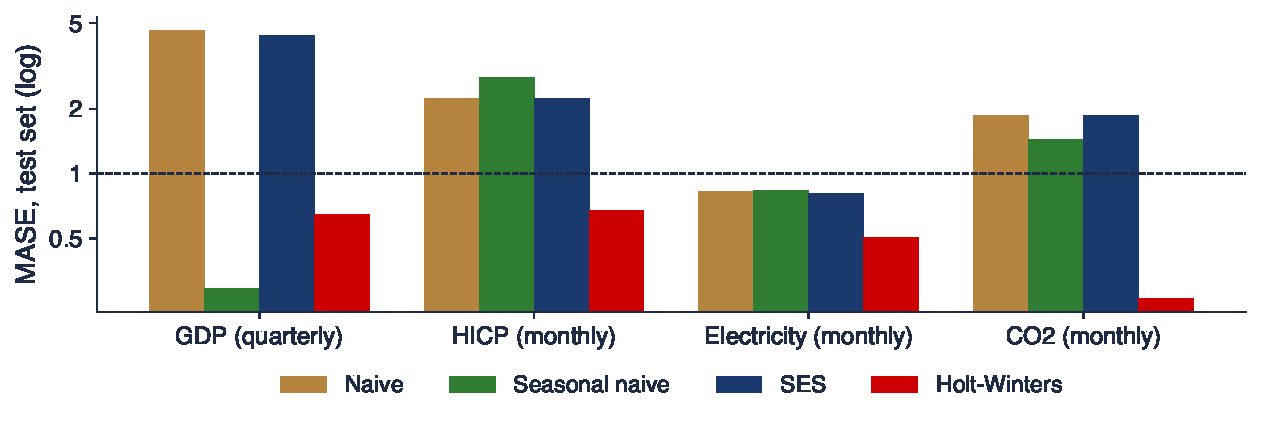
\includegraphics[width=0.94\textwidth,height=0.56\textheight,keepaspectratio]{tsa_ch0_benchmarks.pdf}
\end{center}
\vspace{-2mm}
\begin{itemize}
    \item MASE on the test set (log scale) of four methods on four seasonal series; test sets: the last 8 quarters (GDP) or 24 months; dashed line: MASE = 1
\end{itemize}
\quantlet{TSA\_ch0\_forecast}{\qlurl{TSA_ch0_forecast}}
\end{frame}

\begin{frame}{Interpretation: the Mini-Competition}
\itemsize{\small}
\begin{itemize}
    \item \textbf{Holt--Winters wins on 3 of 4 series}
    \begin{itemize}
        \item CO2: MASE 0.26 against 1.45 for the seasonal naive method; HICP: 0.68 against 2.24 for the naive one
    \end{itemize}
    \item \textbf{GDP: the seasonal naive method wins}, MASE 0.29 against 0.65
    \begin{itemize}
        \item growth stalled in 2025--2026: the trend learnt by Holt--Winters overshoots
    \end{itemize}
    \item \textbf{Naive and SES fail on seasonal series}
    \begin{itemize}
        \item GDP: MASE 4.62 (naive) and 4.39 (SES): they ignore the season
    \end{itemize}
    \item As in M4: no method wins everywhere, and a simple benchmark can beat a better-looking model
\end{itemize}
\end{frame}

\begin{frame}{Recap: forecasts and their evaluation}
\itemsize{\small}
\begin{itemize}
    \item $\hat y_{T+h|T}$ uses only the information up to $T$; uncertainty grows with $h$
    \item Benchmarks: mean, naive, seasonal naive, drift
    \item Split by time; measure MAE, RMSE, MAPE and MASE on the test set only
    \item M4 and our mini-competition: simple methods are strong; combinations and Holt--Winters do well
\end{itemize}
\end{frame}


%=============================================================================
\section{Tools}
%=============================================================================

\begin{frame}{Python for Time Series}
\itemsize{\small}
\begin{itemize}
    \item \textbf{The libraries of the course}
    \begin{itemize}
        \item \textbf{NumPy}: arrays and linear algebra (\refNumpy)
        \item \textbf{pandas}: tables indexed by date, resampling, lags, differences (\refPandas)
        \item \textbf{matplotlib}: charts
        \item \textbf{statsmodels}: decomposition, exponential smoothing, ARIMA, VAR, unit-root tests (\refStatsmodels)
        \item \textbf{arch}: GARCH models (Chapter 5)
    \end{itemize}
    \item \textbf{Google Colab}: notebooks in the browser, nothing to install
    \begin{itemize}
        \item open a course notebook with one click; \emph{File $\to$ Save a copy in Drive} keeps your changes
        \item every chart of the slides has a Quantlet: the same code, runnable in Colab
    \end{itemize}
\end{itemize}
\end{frame}

\begin{frame}[fragile]{A First Script}
\itemsize{\scriptsize}
\begin{columns}[T]
\begin{column}{0.62\textwidth}
\begin{lstlisting}
import pandas as pd
from statsmodels.tsa.seasonal import seasonal_decompose
from statsmodels.tsa.holtwinters import ExponentialSmoothing

# Romanian real GDP, quarterly (Eurostat)
url = ('https://ec.europa.eu/eurostat/api/dissemination/'
       'sdmx/2.1/data/namq_10_gdp/Q.CLV10_MEUR.NSA.B1GQ.RO'
       '?format=SDMX-CSV')
t = pd.read_csv(url)
y = pd.Series(t['OBS_VALUE'].values / 1000,
              index=pd.PeriodIndex(t['TIME_PERIOD'], freq='Q'))
y = y.to_timestamp()

dec = seasonal_decompose(y, model='multiplicative', period=4)
print(dec.seasonal.iloc[:4])            # seasonal factors
yoy = 100 * (y / y.shift(4) - 1)         # annual growth, %
hw = ExponentialSmoothing(y, trend='add', seasonal='mul',
                          seasonal_periods=4).fit()
print(hw.forecast(4))                    # next four quarters
\end{lstlisting}
\end{column}
\begin{column}{0.35\textwidth}
\begin{itemize}
    \item \textbf{Line by line}
    \item read the series directly from the Eurostat API (no key)
    \item \texttt{PeriodIndex}: quarters as the time index
    \item classical multiplicative decomposition with $m = 4$
    \item \texttt{shift(4)}: the value of the same quarter a year earlier
    \item Holt--Winters with additive trend and multiplicative season
    \item API: application programming interface
\end{itemize}
\end{column}
\end{columns}
\end{frame}


%=============================================================================
\section{Possible Contribution of AI}
%=============================================================================

\begin{frame}{Possible Contribution of AI}
\itemsize{\small}
\begin{itemize}
    \item \textbf{Where an AI assistant helps}
    \begin{itemize}
        \item a first draft of the code that reads a Eurostat or BNR series and plots it
        \item explaining an error message or a statsmodels function
        \item listing candidate explanations of a pattern (a drop in GDP, a jump in EUR/RON)
    \end{itemize}
    \item \textbf{Time-series errors that AI code makes often}
    \begin{itemize}
        \item a random train/test split, which lets the model see the future
        \item growth over one quarter called ``annual growth''; \texttt{shift(1)} instead of \texttt{shift(4)}
        \item an RMSE without the square root; a MAPE on a series that crosses zero
    \end{itemize}
    \item Seminar 0, exercise C2: find three such errors in an AI answer
\end{itemize}
\end{frame}

\begin{frame}{Checks Before Trusting a Result}
\itemsize{\small}
\begin{itemize}
    \item \textbf{The data}
    \begin{itemize}
        \item plot the series first; check the frequency, the units, the first and the last date
        \item adjusted or unadjusted? A model for the season needs the unadjusted series
    \end{itemize}
    \item \textbf{The evaluation}
    \begin{itemize}
        \item the test set comes after the training set; it is used once, at the end
        \item compare with the naive and seasonal naive forecasts before claiming success
    \end{itemize}
    \item \textbf{The claims}
    \begin{itemize}
        \item every reference: open the DOI; every number: recompute it
        \item declare the use of AI in \texttt{AI\_USE.md}
    \end{itemize}
\end{itemize}
\end{frame}


%=============================================================================
\section{Conclusions}
%=============================================================================

\begin{frame}{Key Takeaways}
\itemsize{\small}
\begin{itemize}
    \item Grade: 70\% exam, 20\% project, 10\% attendance; AI allowed and declared; seminars before lectures
    \item A time series is ordered in time; its dependence on the past is what makes forecasting possible
    \item Components: trend, seasonality (fixed period), cycle (no fixed period), remainder; additive or multiplicative
    \item Yule and Slutsky: dependence and sums of shocks, the roots of AR and MA models
    \item The ACF reveals trend (slow decay), season (peaks at $m$) and memory
    \item Exponential smoothing weighs the recent past more; evaluate every forecast against naive benchmarks on a test set
\end{itemize}
\end{frame}

\begin{frame}{Self-Assessment, Project Idea, and Next: \tsachlinkt{https://danpele.github.io/Time-Series-Analysis/EN/Courses/chapter1_stochastic_processes_stationarity.pdf}{Chapter 1}}
\itemsize{\footnotesize}
\begin{columns}[T]
\begin{column}{0.52\textwidth}
\begin{itemize}
    \item \textbf{Self-assessment}
    \begin{itemize}
        \item Why is the quarter-on-quarter growth of unadjusted GDP misleading?
        \item What does a seasonal factor of 0.76 for Q1 mean?
        \item What does an estimated $\alpha$ close to 1 say about a series?
        \item Why must the test set come after the training set?
    \end{itemize}
    \item \textbf{Project idea}
    \begin{itemize}
        \item forecast monthly electricity generation in Romania one year ahead; compare the seasonal naive method, Holt--Winters, and STL followed by SES, with a rolling origin
    \end{itemize}
\end{itemize}
\end{column}
\begin{column}{0.44\textwidth}
\begin{itemize}
    \item \textbf{\tsachlink{https://danpele.github.io/Time-Series-Analysis/EN/Courses/chapter1_stochastic_processes_stationarity.pdf}{Chapter 1}: stochastic processes and stationarity}
    \begin{itemize}
        \item What is a stochastic process?
        \item When does a series have a stable mean and variance?
        \item What are white noise and a random walk?
        \item How do we test that autocorrelations are zero?
    \end{itemize}
\end{itemize}
\end{column}
\end{columns}
\end{frame}


%=============================================================================
\section{References}
%=============================================================================

\begin{frame}{References (1/2)}
\itemsize{\tiny}
\begin{itemize}
    \item Box, G.E.P., Jenkins, G.M. (1970). \emph{Time Series Analysis: Forecasting and Control}. Holden-Day; 4th ed.\ with G.C.\ Reinsel: \href{https://doi.org/10.1002/9781118619193}{Wiley (2008)}.
    \item Brockwell, P.J., Davis, R.A. (2016). \href{https://doi.org/10.1007/978-3-319-29854-2}{\emph{Introduction to Time Series and Forecasting}} (3rd ed.). Springer.
    \item Cleveland, R.B., Cleveland, W.S., McRae, J.E., Terpenning, I. (1990). \href{https://www.scb.se/contentassets/ca21efb41fee47d293bbee5bf7be7fb3/stl-a-seasonal-trend-decomposition-procedure-based-on-loess.pdf}{STL: a seasonal-trend decomposition procedure based on loess}. \emph{Journal of Official Statistics}, 6(1), 3--73.
    \item Engle, R.F. (1982). \href{https://doi.org/10.2307/1912773}{Autoregressive conditional heteroscedasticity with estimates of the variance of United Kingdom inflation}. \emph{Econometrica}, 50(4), 987--1007.
    \item Engle, R.F., Granger, C.W.J. (1987). \href{https://doi.org/10.2307/1913236}{Co-integration and error correction: representation, estimation, and testing}. \emph{Econometrica}, 55(2), 251--276.
    \item Gardner, E.S. (1985). \href{https://doi.org/10.1002/for.3980040103}{Exponential smoothing: the state of the art}. \emph{Journal of Forecasting}, 4(1), 1--28.
    \item Hamilton, J.D. (1994). \href{https://doi.org/10.2307/j.ctv14jx6sm}{\emph{Time Series Analysis}}. Princeton University Press.
    \item Harris, C.R., Millman, K.J., van der Walt, S.J., et al.\ (2020). \href{https://doi.org/10.1038/s41586-020-2649-2}{Array programming with NumPy}. \emph{Nature}, 585, 357--362.
    \item Holt, C.C. (1957; reprinted 2004). \href{https://doi.org/10.1016/j.ijforecast.2003.09.015}{Forecasting seasonals and trends by exponentially weighted moving averages}. \emph{International Journal of Forecasting}, 20(1), 5--10.
    \item Huang, C., Petukhina, A. (2022). \href{https://doi.org/10.1007/978-3-031-13584-2}{\emph{Applied Time Series Analysis and Forecasting with Python}}. Springer.
    \item Hyndman, R.J., Athanasopoulos, G. (2021). \href{https://otexts.com/fpp3/}{\emph{Forecasting: Principles and Practice}} (3rd ed.). OTexts.
    \item Hyndman, R.J., Koehler, A.B. (2006). \href{https://doi.org/10.1016/j.ijforecast.2006.03.001}{Another look at measures of forecast accuracy}. \emph{International Journal of Forecasting}, 22(4), 679--688.
    \item Hyndman, R.J., Koehler, A.B., Snyder, R.D., Grose, S. (2002). \href{https://doi.org/10.1016/S0169-2070(01)00110-8}{A state space framework for automatic forecasting using exponential smoothing methods}. \emph{International Journal of Forecasting}, 18(3), 439--454.
\end{itemize}
\end{frame}

\begin{frame}{References (2/2)}
\itemsize{\tiny}
\begin{itemize}
    \item Keeling, C.D. (1960). \href{https://doi.org/10.3402/tellusa.v12i2.9366}{The concentration and isotopic abundances of carbon dioxide in the atmosphere}. \emph{Tellus}, 12(2), 200--203.
    \item Kolmogorov, A.N. (1941). Interpolation and extrapolation of stationary random sequences. English translation in \href{https://doi.org/10.1007/978-94-011-2260-3_28}{\emph{Selected Works of A.N.\ Kolmogorov}, Vol.\ II}, Springer (1992), 272--280.
    \item Makridakis, S., Hibon, M. (2000). \href{https://doi.org/10.1016/S0169-2070(00)00057-1}{The M3-Competition: results, conclusions and implications}. \emph{International Journal of Forecasting}, 16(4), 451--476.
    \item Makridakis, S., Spiliotis, E., Assimakopoulos, V. (2020). \href{https://doi.org/10.1016/j.ijforecast.2019.04.014}{The M4 Competition: 100,000 time series and 61 forecasting methods}. \emph{International Journal of Forecasting}, 36(1), 54--74.
    \item McKinney, W. (2010). \href{https://doi.org/10.25080/Majora-92bf1922-00a}{Data structures for statistical computing in Python}. \emph{Proceedings of the 9th Python in Science Conference}, 56--61.
    \item Seabold, S., Perktold, J. (2010). \href{https://doi.org/10.25080/Majora-92bf1922-011}{Statsmodels: econometric and statistical modeling with Python}. \emph{Proceedings of the 9th Python in Science Conference}, 92--96.
    \item Sims, C.A. (1980). \href{https://doi.org/10.2307/1912017}{Macroeconomics and reality}. \emph{Econometrica}, 48(1), 1--48.
    \item Slutzky, E. (1937). \href{https://doi.org/10.2307/1907241}{The summation of random causes as the source of cyclic processes}. \emph{Econometrica}, 5(2), 105--146.
    \item Wiener, N. (1949). \href{https://doi.org/10.7551/mitpress/2946.001.0001}{\emph{Extrapolation, Interpolation, and Smoothing of Stationary Time Series}}. MIT Press.
    \item Winters, P.R. (1960). \href{https://doi.org/10.1287/mnsc.6.3.324}{Forecasting sales by exponentially weighted moving averages}. \emph{Management Science}, 6(3), 324--342.
    \item Yule, G.U. (1926). \href{https://doi.org/10.2307/2341482}{Why do we sometimes get nonsense-correlations between time-series?} \emph{Journal of the Royal Statistical Society}, 89(1), 1--63.
    \item Yule, G.U. (1927). \href{https://doi.org/10.1098/rsta.1927.0007}{On a method of investigating periodicities in disturbed series, with special reference to Wolfer's sunspot numbers}. \emph{Philosophical Transactions of the Royal Society A}, 226, 267--298.
\end{itemize}
\end{frame}

\end{document}
